%\documentclass[aspectratio=169,notes]{beamer}
\documentclass[aspectratio=169]{beamer}
\usepackage[english]{babel} % just for german

\usepackage[utf8]{inputenc}
\usepackage[scaled]{helvet}

\usepackage[T1]{fontenc}
\usepackage{amsmath,amssymb,amstext}
\usepackage[overlay,absolute]{textpos} % for textboxes
\usepackage{beamerthemesplit}
\usepackage[]{media9}
\usepackage{multimedia} % for videos
\usepackage{graphicx} % not needed in beamer
\usepackage[export]{adjustbox} % align images left,center...
\usepackage{import} % to import images with tex text from inkscape - use path to image
\usepackage{xcolor} % to change textcolor
\usepackage{hyperref}
\usepackage{booktabs}
\usepackage{setspace}
\usepackage{siunitx}
\usepackage{upgreek}
\usepackage{mathrsfs}
\usepackage{subfig}
\usepackage{caption}
\usepackage{multirow}
\usepackage{tcolorbox}
\usepackage{epstopdf}
\usepackage{pdfcomment}
\usepackage{cancel} % to cross out
\newcommand\Ccancel[2][black]{\renewcommand\CancelColor{\color{#1}}\cancel{#2}}
\usepackage{tikz}
\usetikzlibrary{tikzmark}
\usetikzlibrary{arrows}
\usetheme{Boadilla} %{Pittsburgh} %{boxes} %{Boadilla}

%%% uncomment to add notes - final step when presentation is ready
%\usepackage{pgfpages}
%\setbeamertemplate{note page}[plain]
%\setbeameroption{show notes on second screen}


%% set color box 
%\tcbset{highlight math style={colframe=red,colback=white}}

% length scale for text positions
\setlength{\TPHorizModule}{\paperwidth}
\setlength{\TPVertModule}{\paperheight}



% colors definitions
\definecolor{royalblue}{RGB}{65,105,255}	% 4169ff
\definecolor{darkblue}{RGB}{0,0,153}		% 000099
\definecolor{navy}{RGB}{0,0,128}			% 000080
\definecolor{blue1}{RGB}{0,102,204}			% 0066cc
\definecolor{cyan0}{RGB}{0,255,255}			% 00ffff
\definecolor{red0}{RGB}{255,0,0}			% ff0000
\definecolor{orange0}{RGB}{255,128,0}		% ff8000
\definecolor{violet}{RGB}{159,64,255}		% 7f00ff
%\definecolor{yellow0}{RGB}{255,255,0}		% ffff00
\definecolor{green1}{RGB}{76,153,0}			% 4c9900
\definecolor{darkgreen}{RGB}{0,126,0}		% 007e00	
\definecolor{pink}{RGB}{204,0,126}			% cc0066
\definecolor{lightblue}{RGB}{153,204,255}

% colors for model functions in beam hardening paper in HEX-format
\definecolor{BS}{HTML}{007e00} 
\definecolor{Yu1}{HTML}{cc00cc}
\definecolor{Yu2}{HTML}{6600cc}  
\definecolor{KS}{HTML}{66cc00} 
\definecolor{MU}{HTML}{ff8000} 
\definecolor{BA}{HTML}{0066cc}

% get rid of bottom navigaiton bars
\setbeamertemplate{footline}{}
% get rid of navigation symbols
\setbeamertemplate{navigation symbols}{}
\setbeamercolor{frametitle}{fg=blue1} % set color of title
\setbeamercolor{footline}{fg=blue1}
\setbeamerfont{footline}{series=\bfseries}
%\setbeamerfont{footline}{\large}

\includeonly{%
%Title,
%Motivation,
BeamHardening,
%X-DFA,
%SedimentingBed,
%BackupSlides
}


\begin{document}
\begin{frame}[noframenumbering,plain]

\begin{tikzpicture}[remember picture,overlay]
\fill[blue1]
(current page.north west) rectangle ([xshift=-12.cm,yshift=-10.cm]current page.east|-{pic cs:end});
\end{tikzpicture}

\begin{textblock}{0.22}(0.02,0.06)
	
\includegraphics[width=\textwidth]{Sources/title/Logo_FAU_DinA4_RGB_Negativ.png}
%		\vspace{2cm}
	
\includegraphics[width=\textwidth]{Sources/title/mss_negative.png}
	\vspace{1.5cm}
\end{textblock}
\begin{textblock}{0.25}(0.05,0.45)
	\textcolor{white}{
	{\large PhD defense \\
		\textbf{Manuel Baur}}}
\end{textblock}

\begin{textblock}{0.23}(0.01,0.7)
	\centering
	\begin{spacing}{.9}
		\textcolor{white}{
		\footnotesize{
			{\setstretch{.1}
			Funded by the German Federal Ministry for Economic Affairs and Energy,
			grant no.\ 50WM 1653}
			}
		}
	\end{spacing}
\end{textblock}



% make title
\begin{textblock}{0.65}(0.3,0.05)
	\begin{center}
		\textcolor{blue1}{							
		\Large{\textbf{
			X-ray radiography of granular systems\\
			-- particle densities and dynamics}}
		}
	\end{center}
\end{textblock}


\begin{textblock}{0.4}(0.3,0.25)
	\centering
	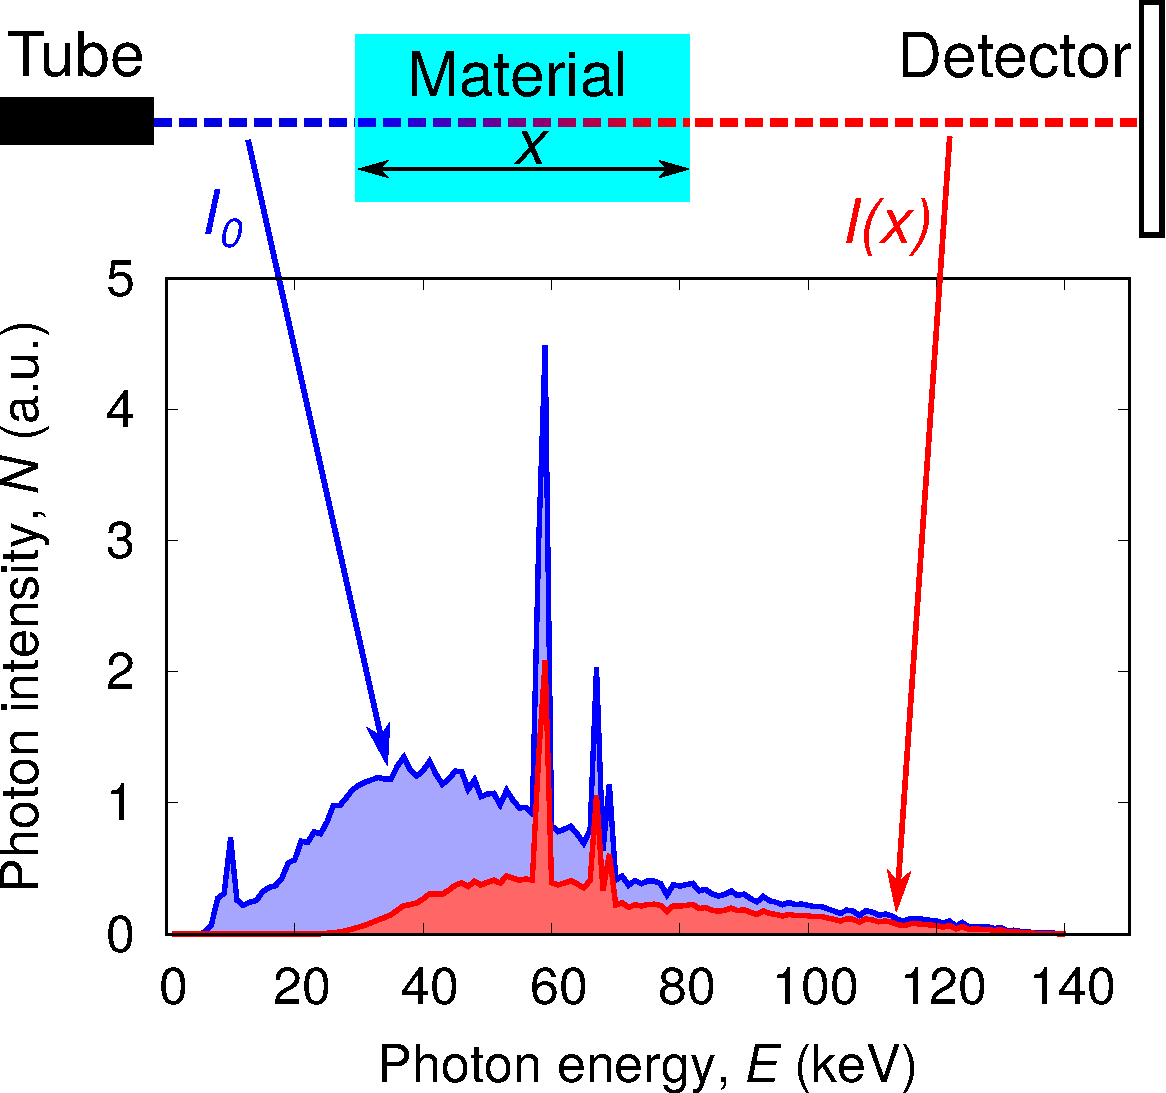
\includegraphics[width=\textwidth]
	{Sources/beam_hardening/x-ray_spectra_beam_hardening.pdf}
%	{Sources/beam_hardening/N_spectrum_after_material_filled_curves.eps}
\end{textblock}
	
\begin{textblock}{0.25}(0.72,0.35)
	\centering
	\centering
	\movie[width =\textwidth, poster, loop]
	{
\includegraphics[width=\textwidth]{Sources/X-DFA/cropped_80kV_340uA_38ms_0000.png}}
	{Sources/X-DFA/3500mul_per_min_cropped_roi_512x512.avi}
\end{textblock}

\end{frame}




%%% start from here on with frame numbers
\addtobeamertemplate{navigation symbols}{}{%
	\usebeamerfont{footline}%
	\usebeamercolor[fg]{footline}%
	\hspace{1em}%
	\footnotesize
	\insertframenumber %/\inserttotalframenumber
}



%%%%% MOTIVATION & INTRODUCTION
\frame{
\begin{tikzpicture}[remember picture,overlay]
\fill[blue1]
(current page.north west) rectangle ([xshift=0.55\paperwidth,yshift=0.27\paperheight]current page.west|-{pic cs:end});
\end{tikzpicture}
\begin{textblock}{0.55}(0.02,0.03)
	\textcolor{white}{							
	\Large{X-ray radiography of granular systems \\
		-- particle densities and dynamics}
	}
\end{textblock}

\begin{textblock}{0.15}(0.05,0.2)
\includegraphics[width=\textwidth]{Sources/motivation/sand.png}
\\[0.2cm]
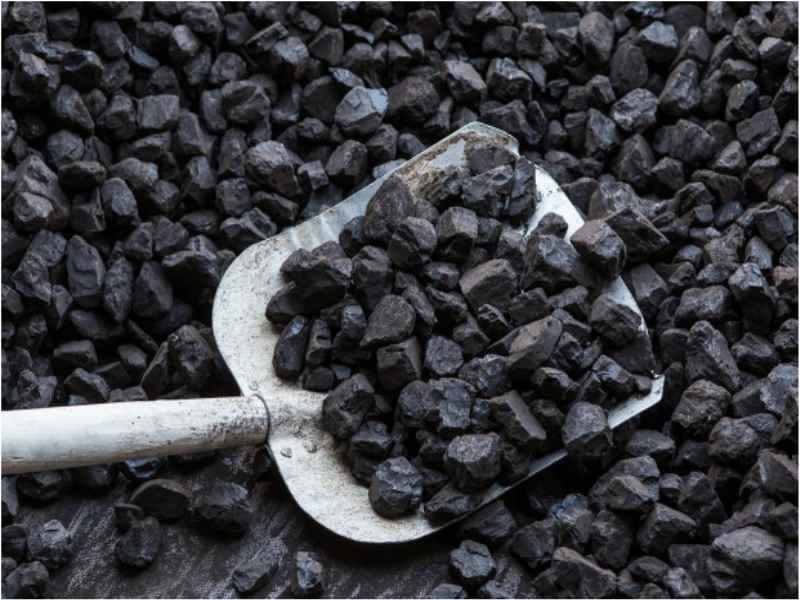
\includegraphics[width=\textwidth]{Sources/motivation/coal.png}
\\[0.2cm]
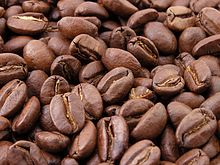
\includegraphics[width=\textwidth]{Sources/motivation/coffee.png}
{\Huge$\vdots$}
\end{textblock}

\begin{textblock}{0.35}(0.25,0.2)
\visible<2->{
\centering
\textbf{Granular materials are athermal}\\[0.1cm]
\begin{minipage}[c]{0.25\textwidth}
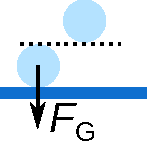
\includegraphics[width=\textwidth]{Sources/motivation/lift_particle.pdf}
\end{minipage}
\hfill
\begin{minipage}[c]{0.6\textwidth}
\begin{align}
E_\text{pot} &\approx \textcolor{red}{10^{10}} E_\text{thermal}\nonumber
\end{align}
\end{minipage}
}
\end{textblock}

\begin{textblock}{0.35}(0.25,0.5)
\centering
\visible<4->{
\textbf{Dissipative interactions}\\[0.1cm]
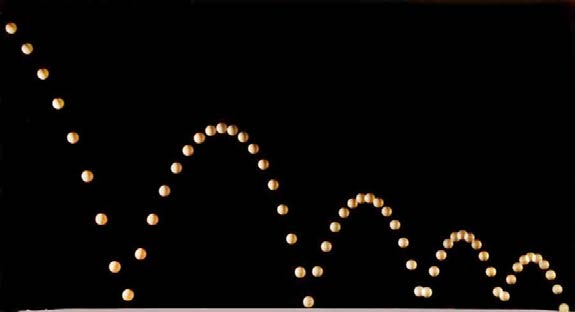
\includegraphics[width=\textwidth]{Sources/motivation/Driscoll_et_al_2016.png}\\
{\scriptsize Driscoll \textit{et al} (2016)}}
\end{textblock}

\begin{textblock}{0.25}(0.7,0.1)
\centering
\visible<3->{
\textbf{Volume fraction} 
\[\Phi = \frac{V_\text{Particles}}{V_\text{Container}}\]}
\only<3>{
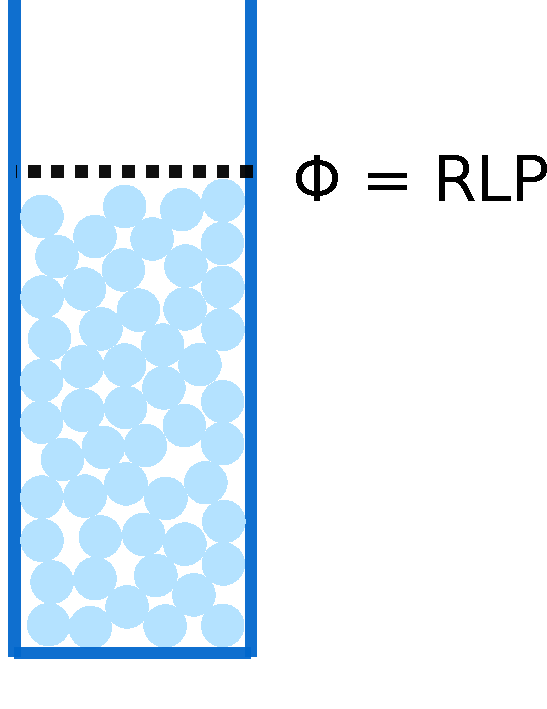
\includegraphics[width=\textwidth]{Sources/motivation/setup-fluidized_bed_sedimented.pdf}}
\only<4,5>{
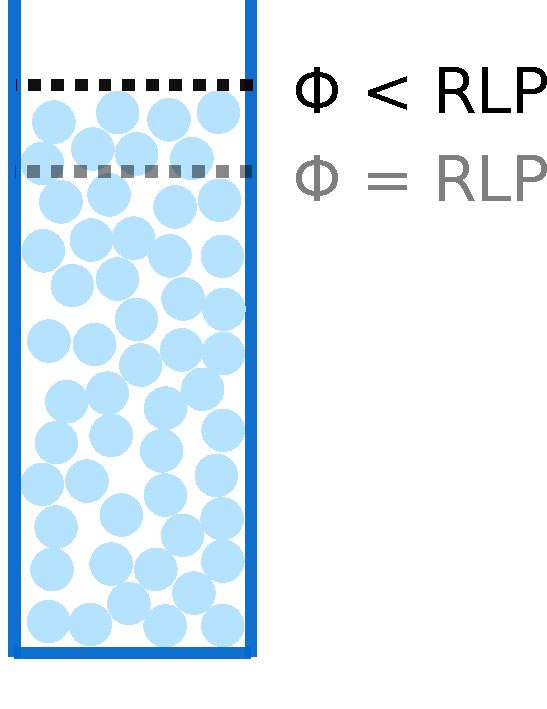
\includegraphics[width=\textwidth]{Sources/motivation/setup-fluidized_bed_expanded.pdf}}
\end{textblock}
}



%%%%% Motivation fluidized bed
\frame{
\begin{tikzpicture}[remember picture,overlay]
\fill[blue1]
(current page.north west) rectangle ([xshift=0.55\paperwidth,yshift=0.27\paperheight]current page.west|-{pic cs:end});
\end{tikzpicture}
\begin{textblock}{0.55}(0.02,0.03)
	\textcolor{white}{							
		\Large{X-ray radiography of granular systems \\
			-- particle densities and dynamics}
	}
\end{textblock}
	
\begin{textblock}{0.55}(0.02,0.2)
\visible<1->{
	\textbf{Liquid fluidized bed}\\[0.5cm]
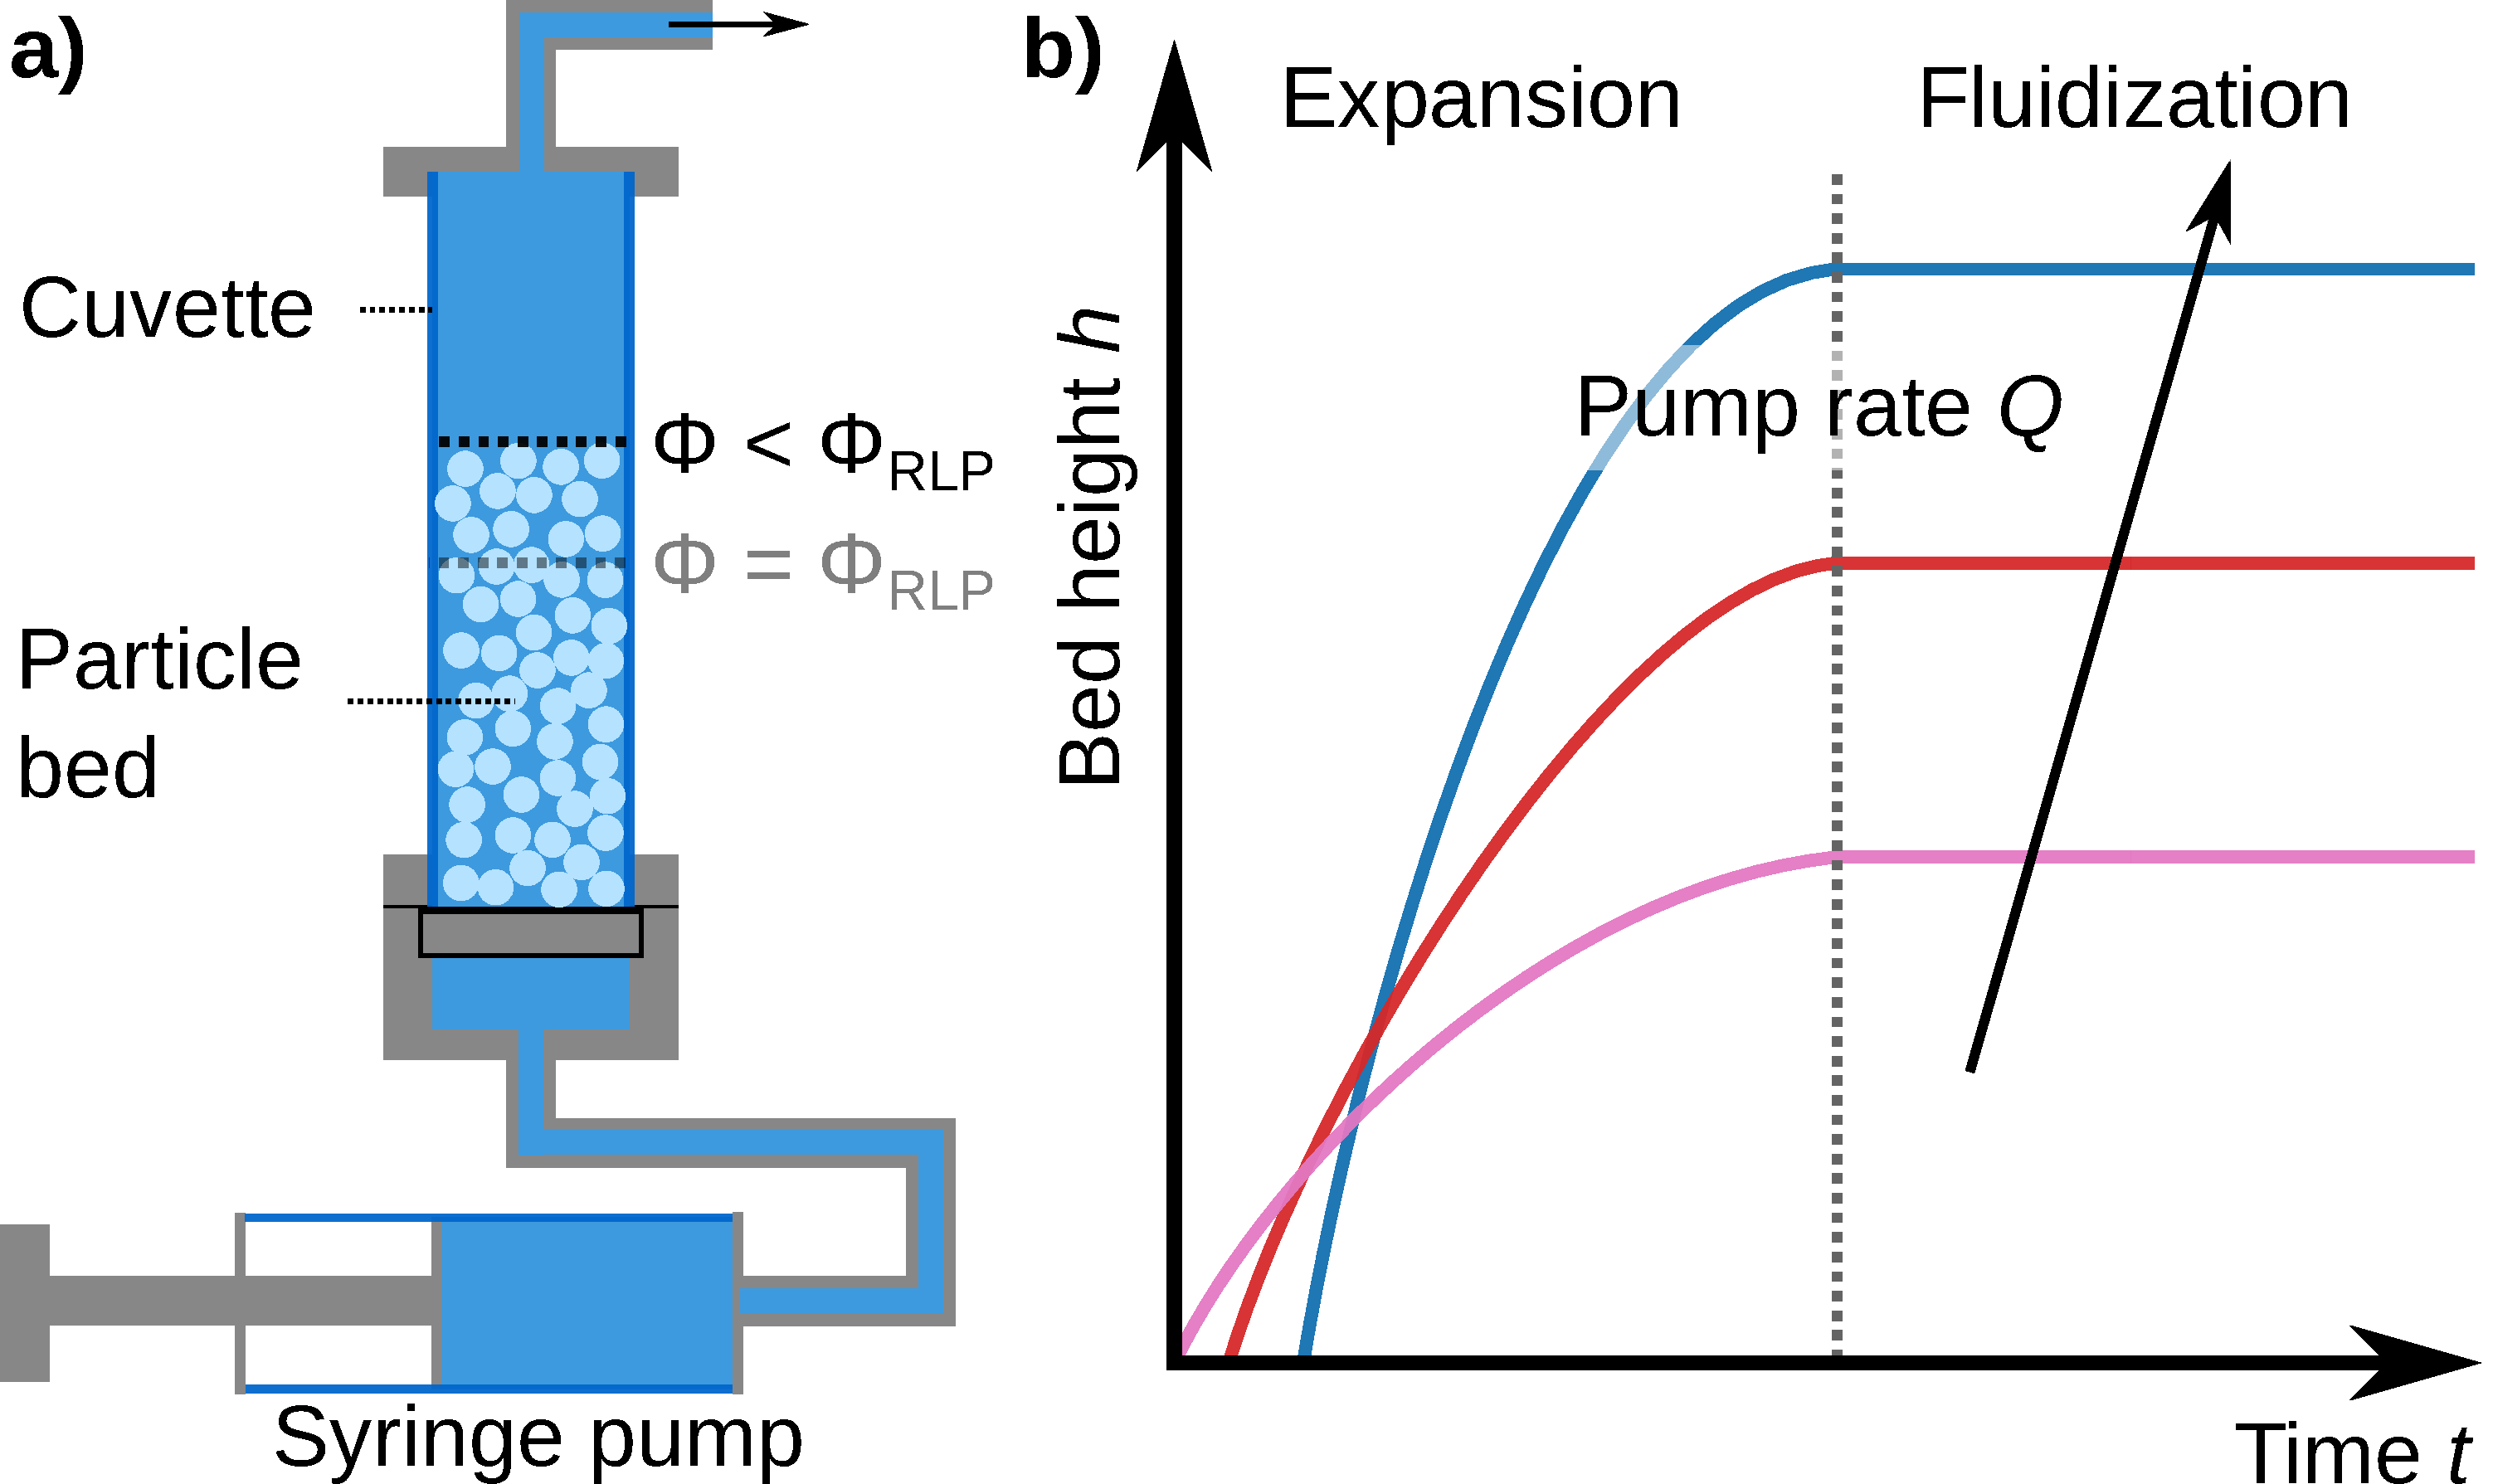
\includegraphics[width=\textwidth]{Sources/motivation/setup-fluidized_bed_final.pdf}}
\end{textblock}

\begin{textblock}{0.5}(0.55,0.1)
	\centering
	\visible<2->{
	\movie[height=0.75\textheight,loop]
	{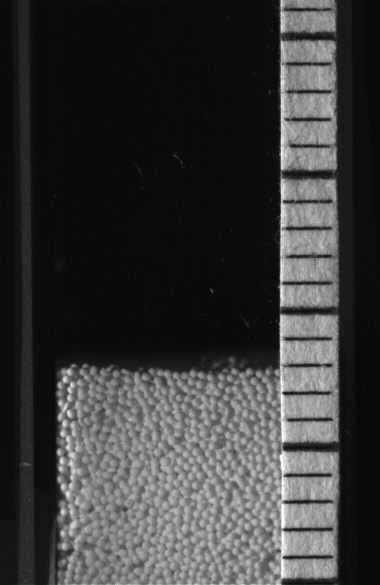
\includegraphics[height=0.75\textheight]{Sources/motivation/video_welm_paetzold.png}}	
	{videos/video_welm_paetzold.avi}
	
	{\footnotesize Master thesis Welm Pätzold}\\[0.2
	cm]
	
	\textcolor{red}{Particulate flows are \textbf{opaque}}}
\end{textblock}
}



%% X-RAY RADIOGRAPHY
\frame{
\begin{tikzpicture}[remember picture,overlay]
\fill[blue1]
(current page.north west) rectangle ([xshift=0.46\paperwidth,yshift=0.33\paperheight]current page.west|-{pic cs:end});
\end{tikzpicture}

\begin{textblock}{0.5}(0.02,0.03)
	\textcolor{white}{
		\Large X-ray radiography \& tomography}
\end{textblock}

\begin{textblock}{0.7}(0.02,0.05)
	\centering
	\only<1>{
	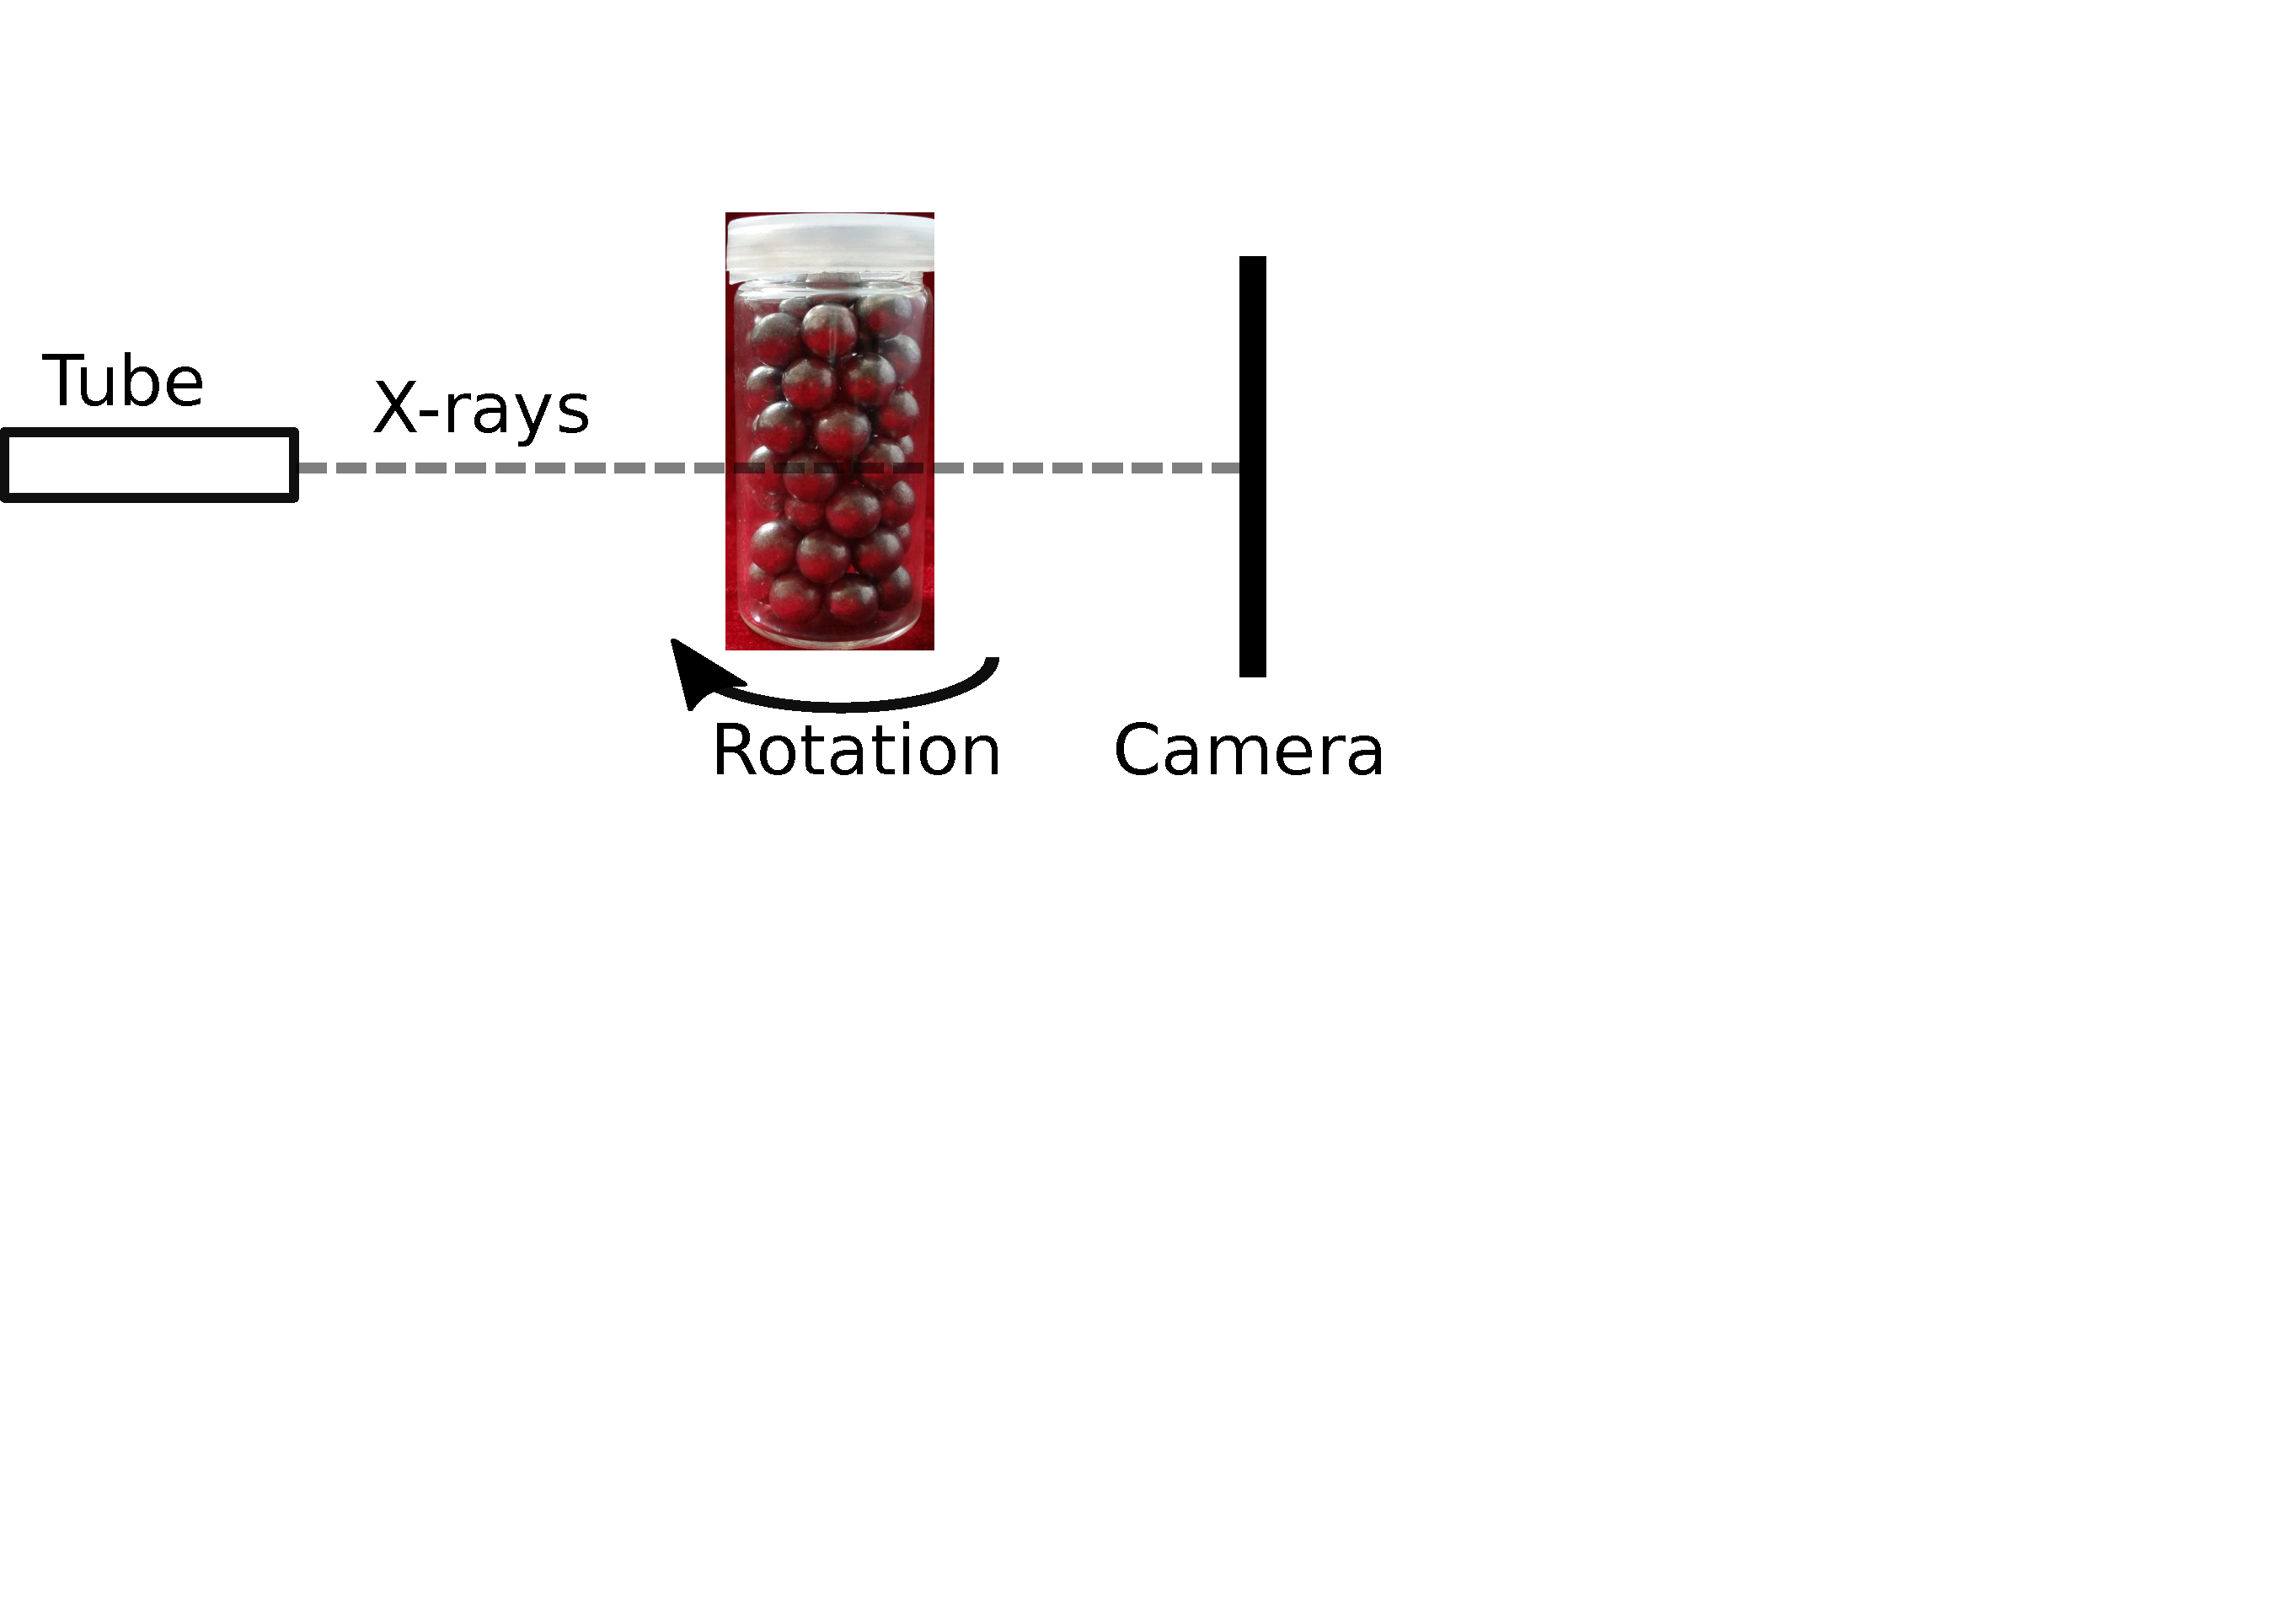
\includegraphics[width=\textwidth]{Sources/motivation/x-ray_setup_use0.pdf}}
	\visible<2->{
	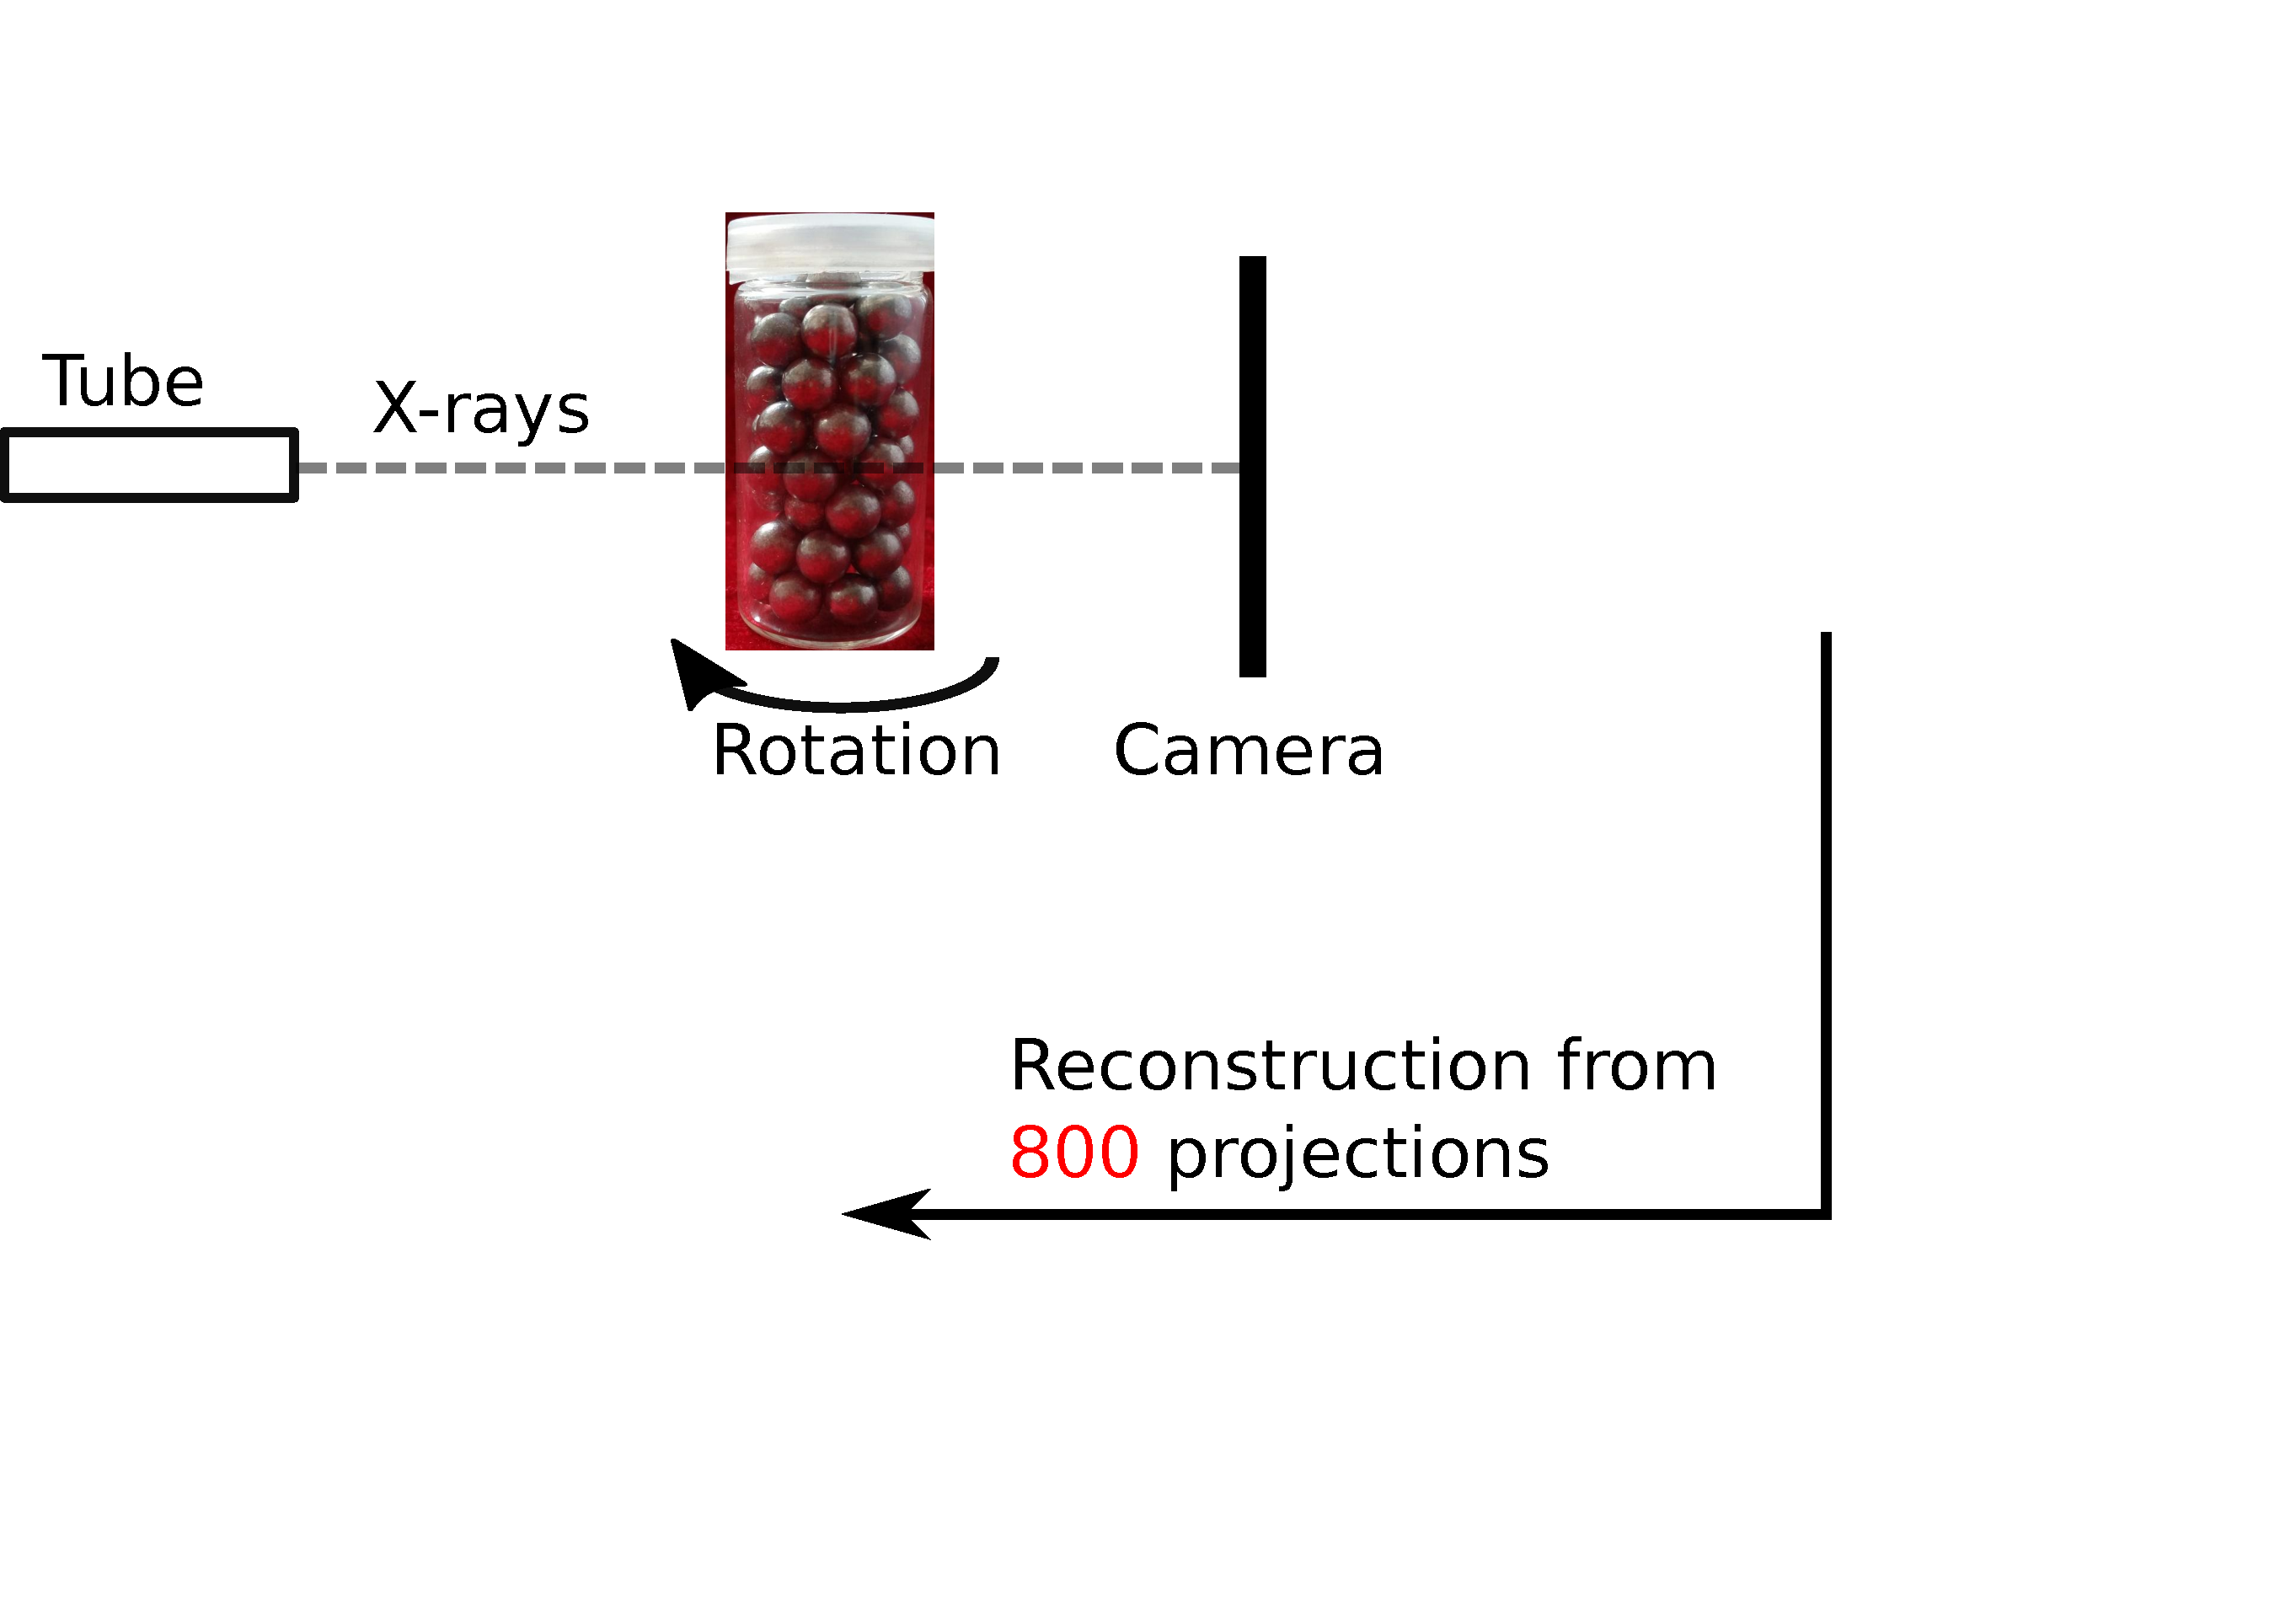
\includegraphics[width=\textwidth]{Sources/motivation/x-ray_setup_use.pdf}}
\end{textblock}

%% Video of Projections
\begin{textblock}{0.22}(0.45,0.06)
	\visible<1->{
	\centering
	Radiogram\\
	\fbox{\parbox{\textwidth}{
	\movie[width =\textwidth,loop]
	{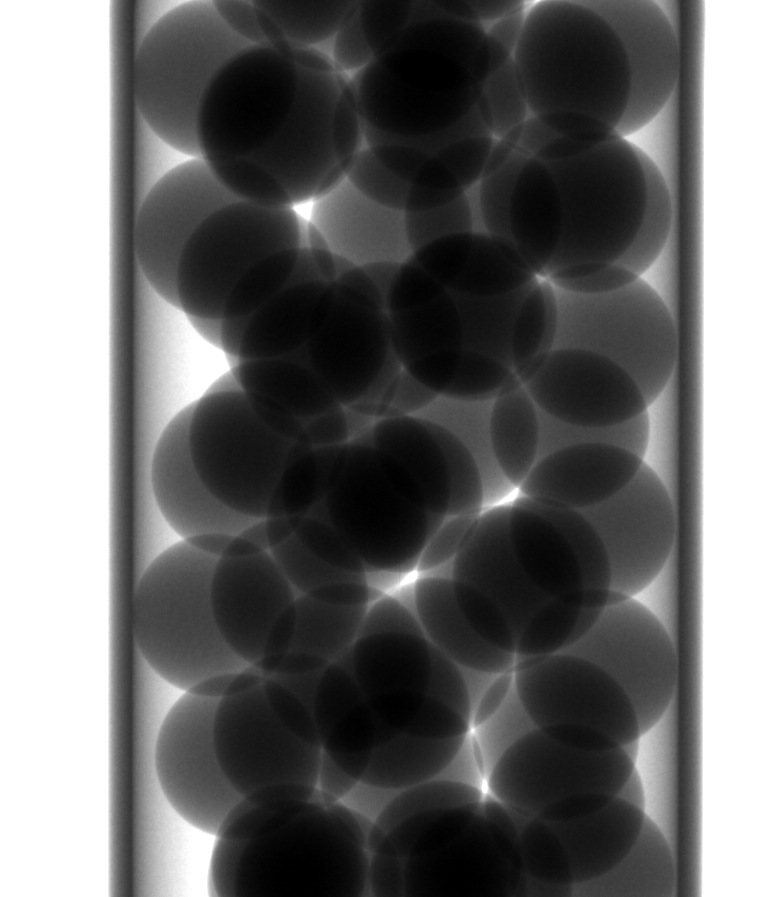
\includegraphics[width=\textwidth]{Sources/motivation/Projection0000.png}}
	{videos/Projections360degree.avi}}}}
\end{textblock}

\begin{textblock}{0.28}(0.7,0.25)
	\visible<1->{
	2D projections of 3D object\\
	\textcolor{blue1}{Short} acquisition time}\\
	$\rightarrow$ \textcolor{blue1}{Dynamic} system
\end{textblock}

% Video of Tomography
\begin{textblock}{0.2}(0.05,0.48)
	\visible<2->{
	\centering
	Tomogram\\
	\movie[width =\textwidth,loop]
	{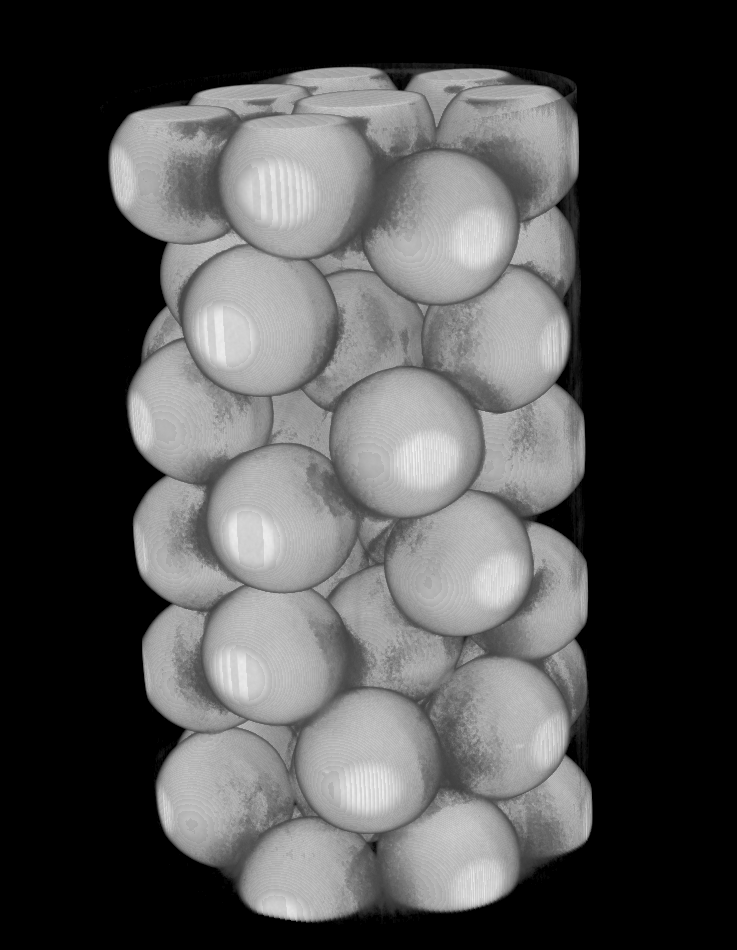
\includegraphics[width=\textwidth]{Sources/motivation/Images_tomo_movie0000.png}}
	{videos/tomogram_360degree.avi}}
\end{textblock}

\begin{textblock}{0.5}(0.27,0.8)
	\visible<2->{
	Full 3D information\\
	\textcolor{red}{Long} acquisition time\\
	$\rightarrow$ \textcolor{red}{Static} objects}
\end{textblock}
}




\frame{
\begin{tikzpicture}[remember picture,overlay]
\fill[blue1]
(current page.north west) rectangle ([xshift=12.cm,yshift=-10.cm]current page.east|-{pic cs:end});
\end{tikzpicture}
\begin{textblock}{0.9}(0.05,0.08)
\centering
\Huge{
\textcolor{white}{Measuring the volume fraction of \textbf{dynamic} granular systems}}\\
\end{textblock}

\begin{textblock}{0.9}(0.05,0.34)
	\centering
	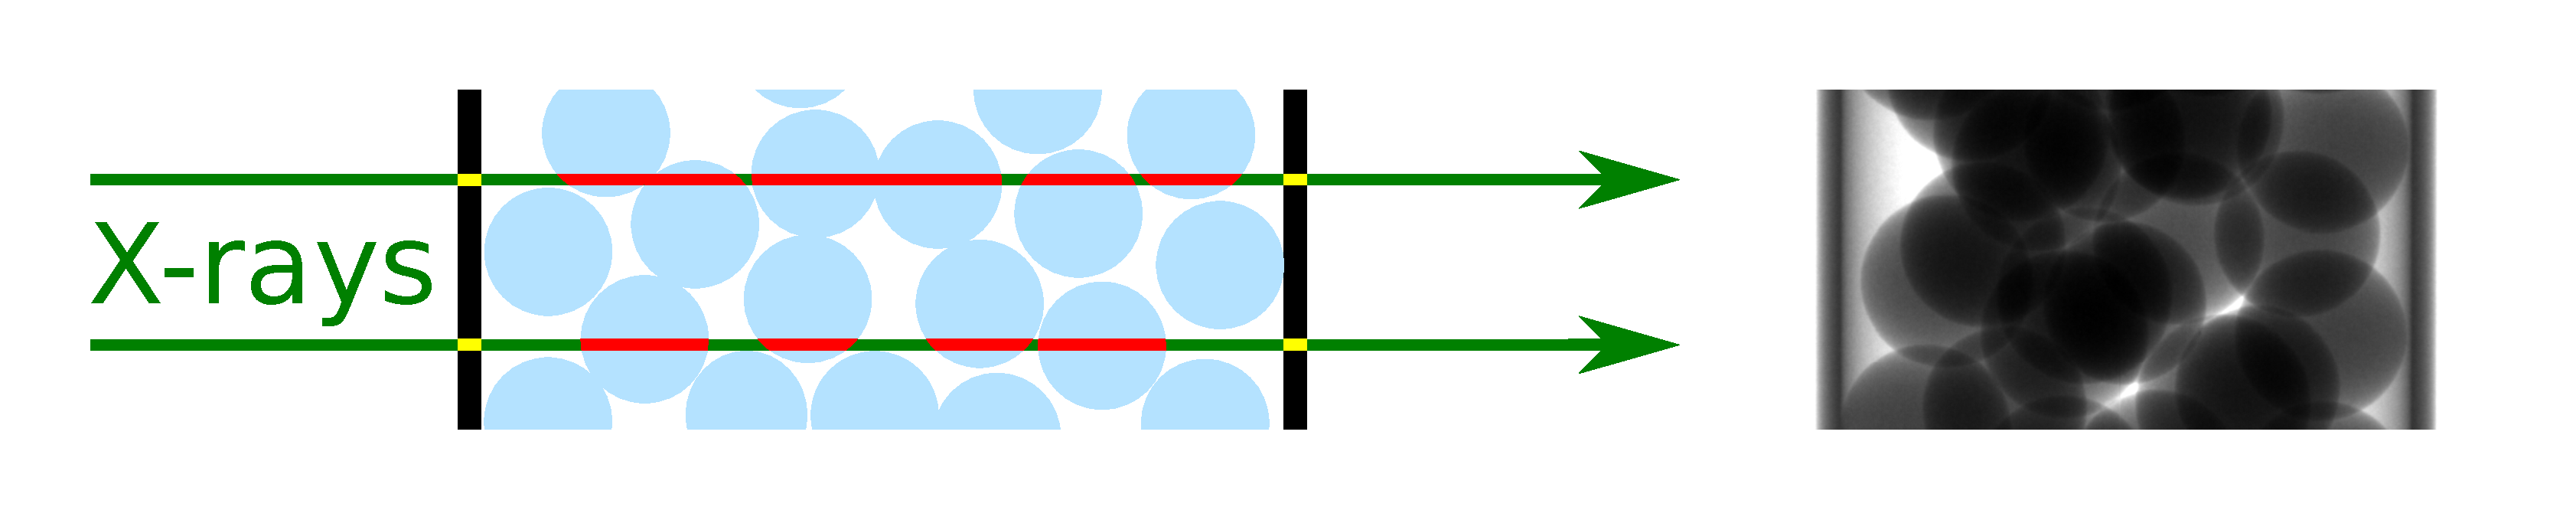
\includegraphics[width=0.8\textwidth]{Sources/beam_hardening/2beams_attenuation_marked.pdf}
\end{textblock}

\begin{textblock}{0.9}(0.05,0.65)
\visible<1->{
\centering
\Huge{
	\textcolor{white}{Correction of beam hardening \\
		in X-ray radiograms}}}
\end{textblock}

\begin{textblock}{0.9}(0.05,0.9)
	\visible<1->{
	\centering
	{
	\textcolor{white}{
		Baur \textit{et al}, \textit{Rev.\ Sci.\ Instrum.}\ (2019)\\
		In collaboration with Norman Uhlmann, Fraunhofer EZRT}}}
\end{textblock}
}


%% ------------------ ATTENUATION OF X-RAYS -----------------------
\frame{
\begin{tikzpicture}[remember picture,overlay]
\fill[blue1]
(current page.north west) rectangle ([xshift=0.33\paperwidth,yshift=0.33\paperheight]current page.west|-{pic cs:end});
\end{tikzpicture}

\begin{textblock}{0.5}(0.02,0.03)
	\textcolor{white}{
		\Large Attenuation of X-rays}
\end{textblock}

\begin{textblock}{0.45}(0.5,0.1)
\centering
Beer-Lambert's law\\[0.2cm]
\visible<1>{
$\textcolor{red}{I(x)} = \textcolor{blue}{I_0} \exp(- \mu\, x)$\\
Thickness: $x = - \frac{1}{\mu} \ln\frac{I(x)}{I_0}$}
\end{textblock}

\begin{textblock}{0.45}(0.5,0.1)
\centering
Beer-Lambert's law\\[0.2cm]
\visible<2->{
$\mu \neq \text{const}$\\
$\textcolor{red}{I(x)} = \textcolor{blue}{I_0} \exp(- \textcolor{darkgreen}{\mu(E,Z,\rho)}\, x)$\\
Thickness: \colorbox{red}{$x =\, ?$}}
\end{textblock}

\begin{textblock}{0.48}(0.5,0.3)
	\visible<2->{
	\centering
	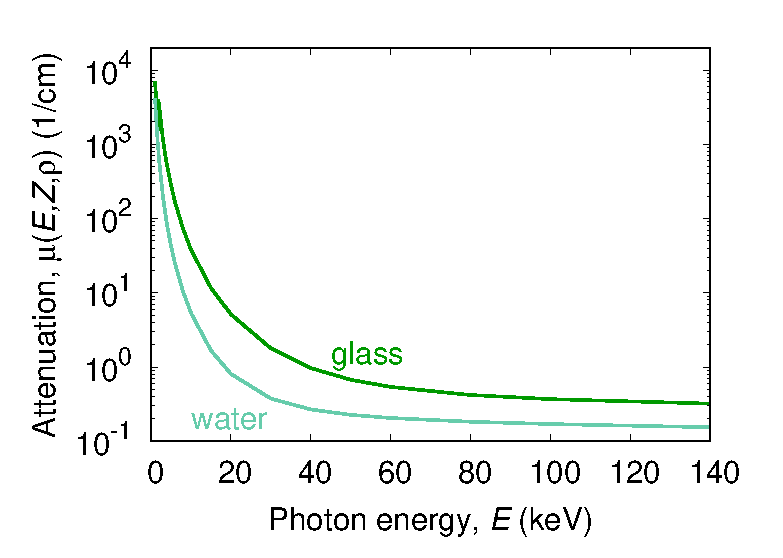
\includegraphics[width=\textwidth]
	{Sources/beam_hardening/Attenuation_vs_energy.eps}}
\end{textblock}
\begin{textblock}{0.48}(0.5,0.9)
	\centering
	\visible<2->{\scriptsize{
		\url{https://www.nist.gov/pml/x-ray-mass-attenuation-coefficients}}}
\end{textblock}

\begin{textblock}{0.45}(0.03,0.14)
	\centering
	\only<1> {%% image of beam through material
	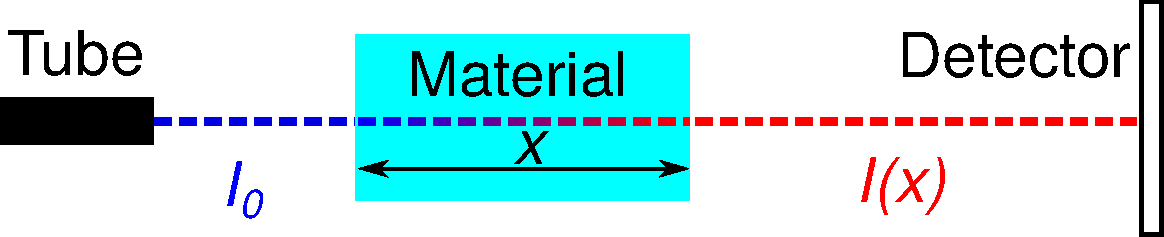
\includegraphics[width=\textwidth]
	{Sources/beam_hardening/beam_through_material.pdf}}
	\only<2>{
	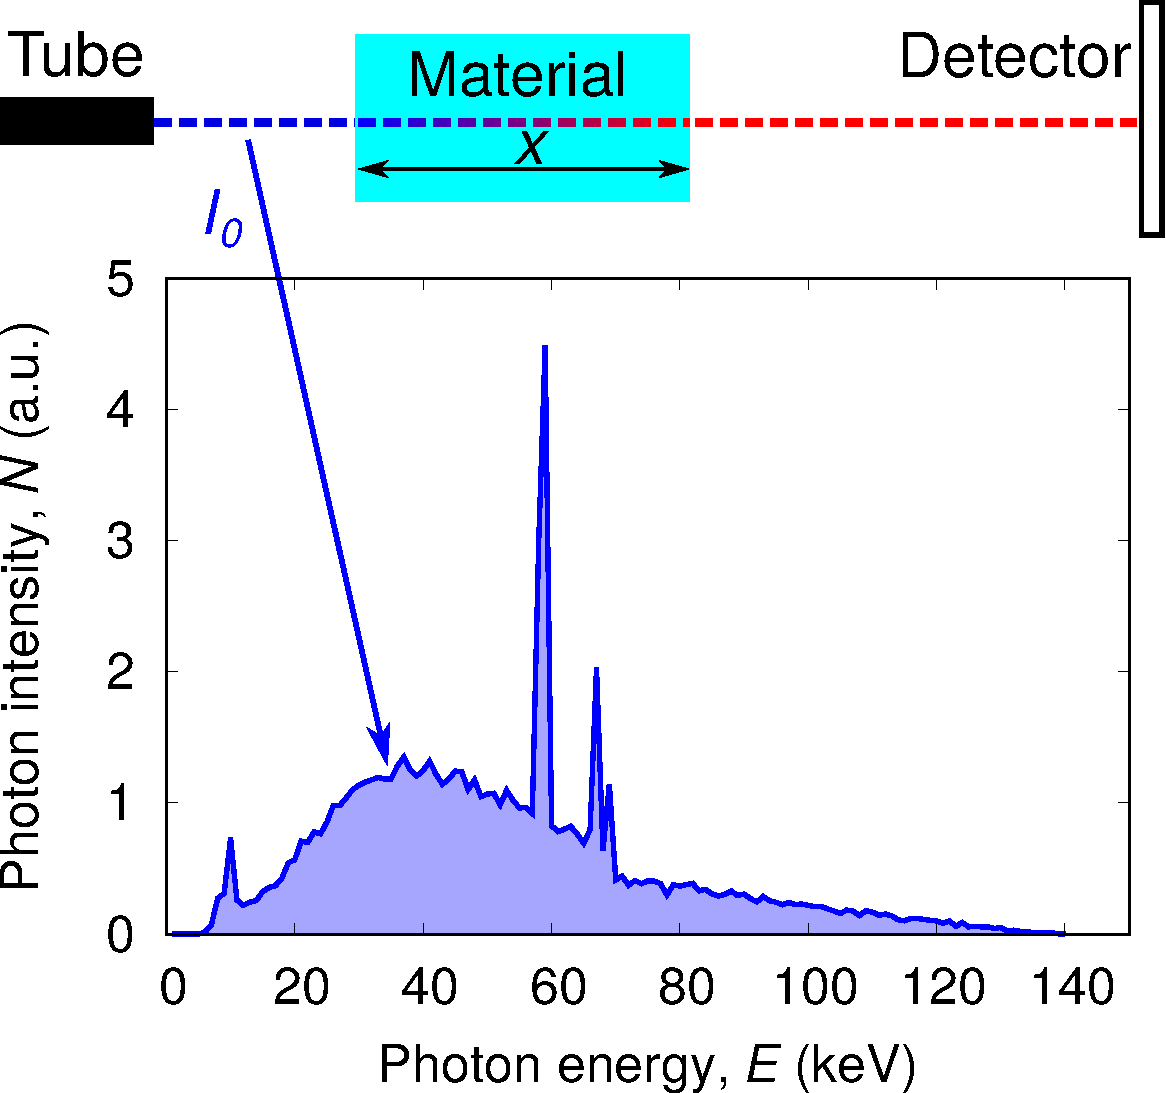
\includegraphics[width=\textwidth]
	{Sources/beam_hardening/x-ray_spectrum_N0.pdf}}
	\only<3>{
	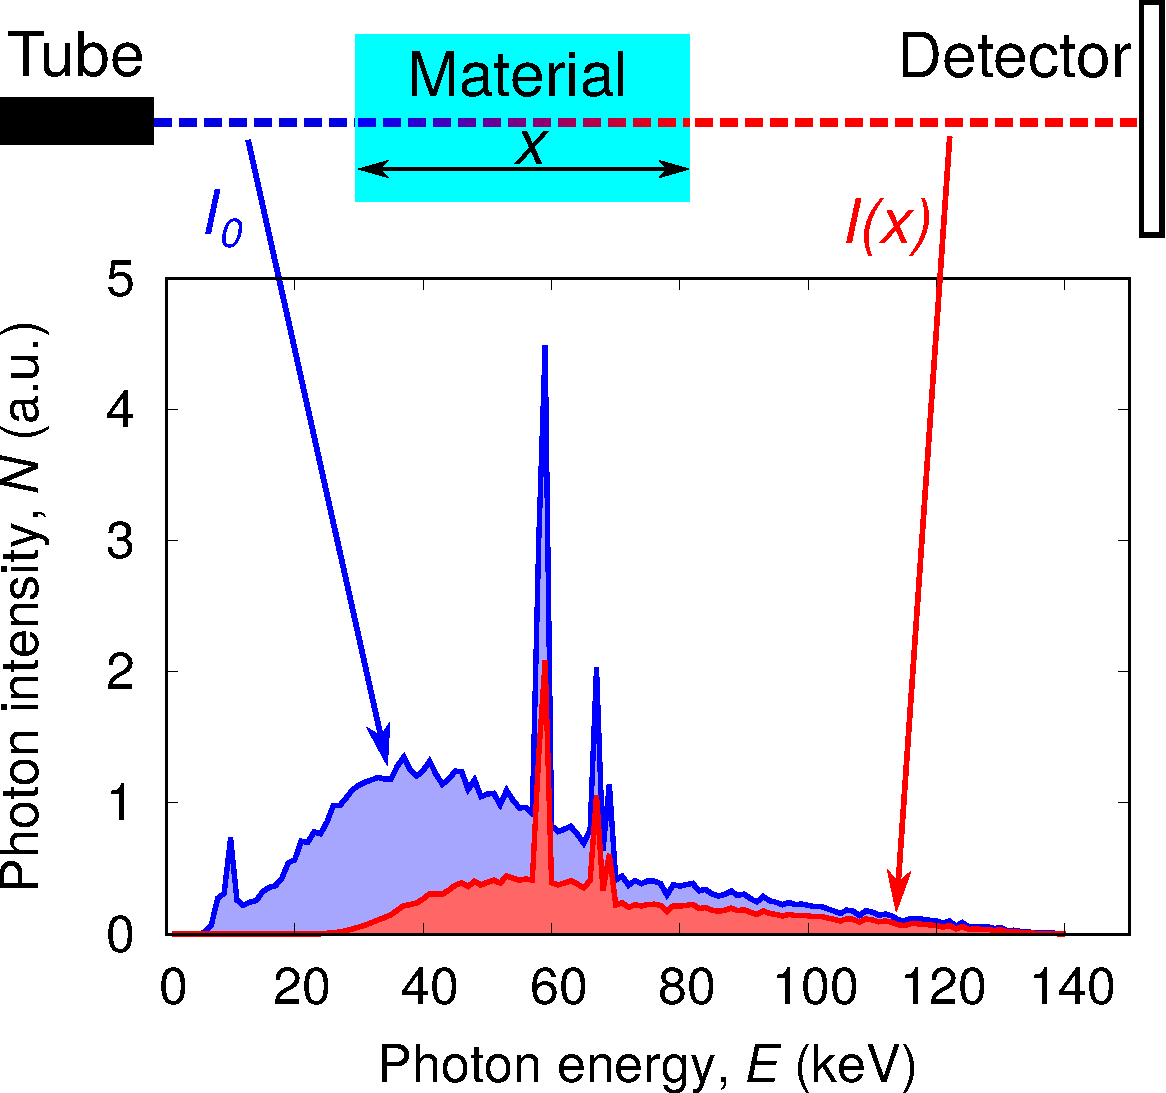
\includegraphics[width=\textwidth]
	{Sources/beam_hardening/x-ray_spectra_beam_hardening.pdf}}
\end{textblock}
\begin{textblock}{0.45}(0.035,0.36)
	\centering
	\only<3>{
	\colorbox{red}{Beam hardening}}
\end{textblock}

}




%%%-------------- The effective attenuation ----------------
\frame{
\begin{tikzpicture}[remember picture,overlay]
\fill[blue1]
(current page.north west) rectangle ([xshift=0.48\textwidth,yshift=0.33\textheight]current page.west|-{pic cs:end});
\end{tikzpicture}

\begin{textblock}{0.5}(0.02,0.03)
	\textcolor{white}{
		\Large The effective attenuation, $\mu_\text{eff}(x)$}
\end{textblock}


\begin{textblock}{0.45}(0.03,0.1)
	\centering
	\only<1>{
	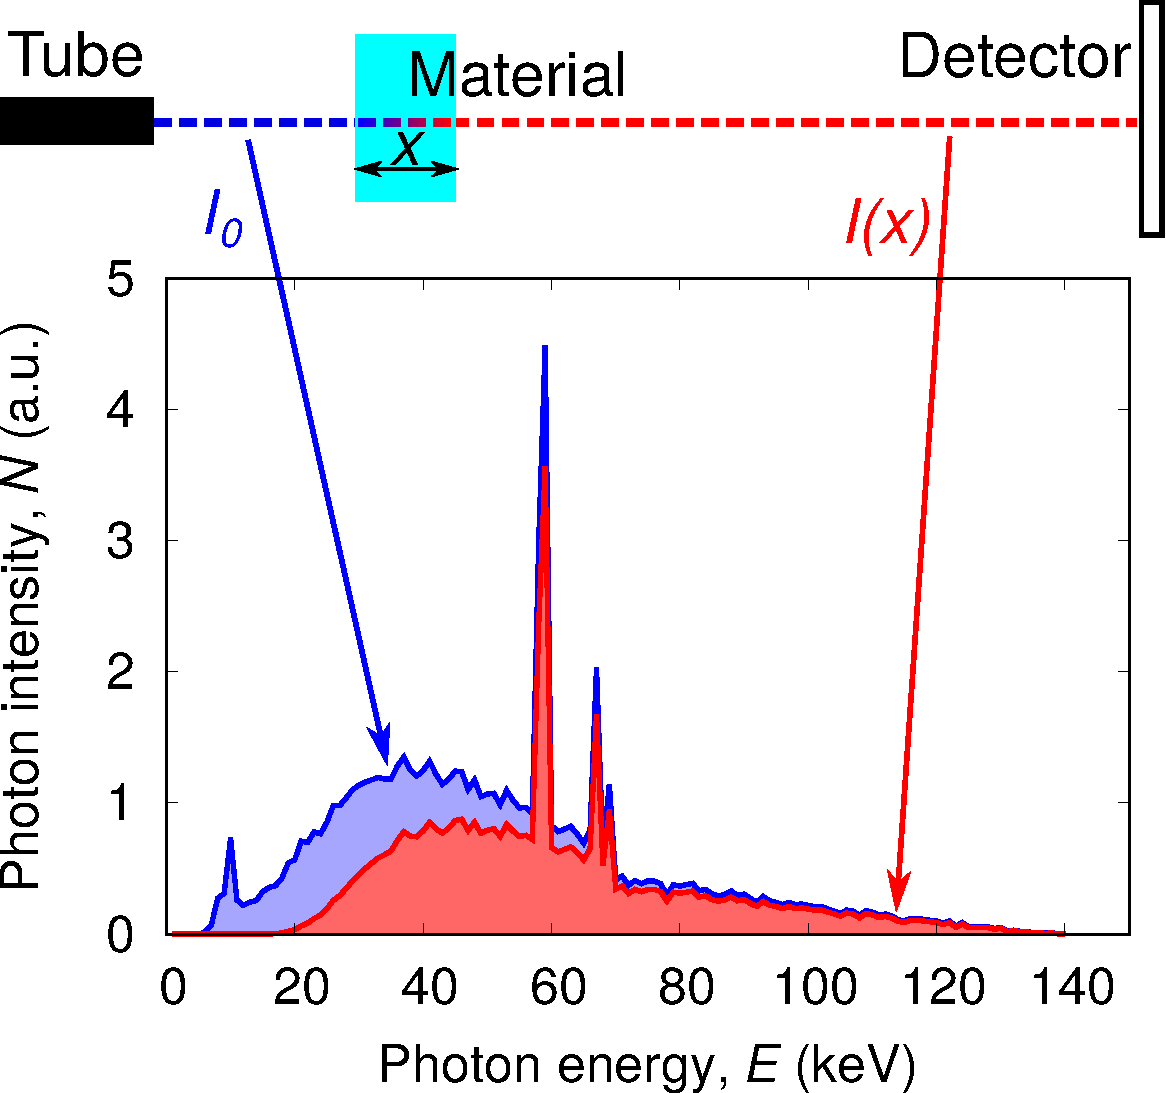
\includegraphics[width=\textwidth]
	{Sources/beam_hardening/x-ray_spectra_beam_hardening_step1.pdf}}
	\only<2>{
	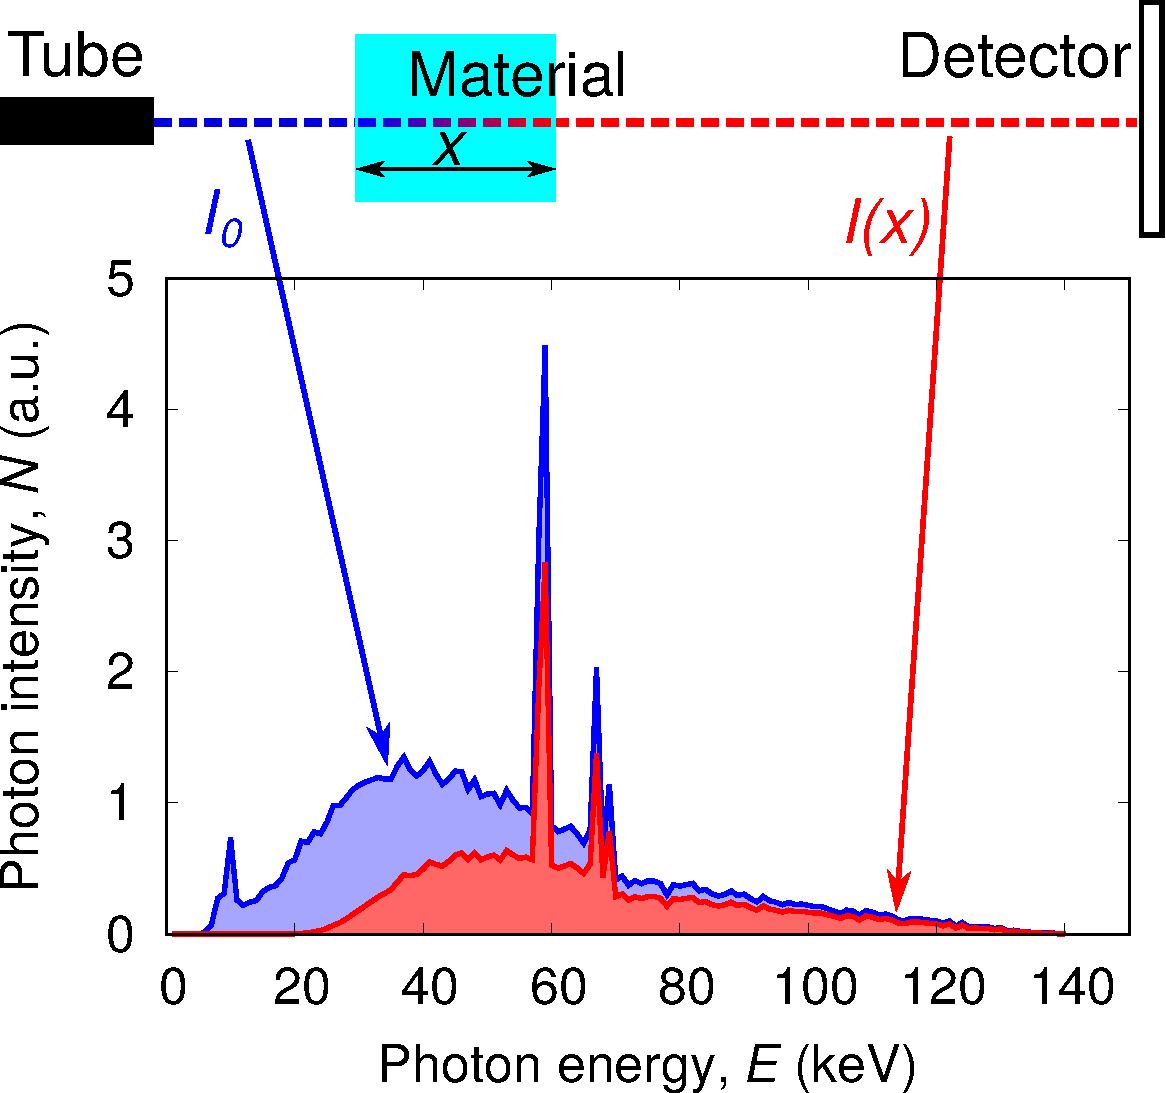
\includegraphics[width=\textwidth]
	{Sources/beam_hardening/x-ray_spectra_beam_hardening_step2.pdf}}
	\only<3,4>{
	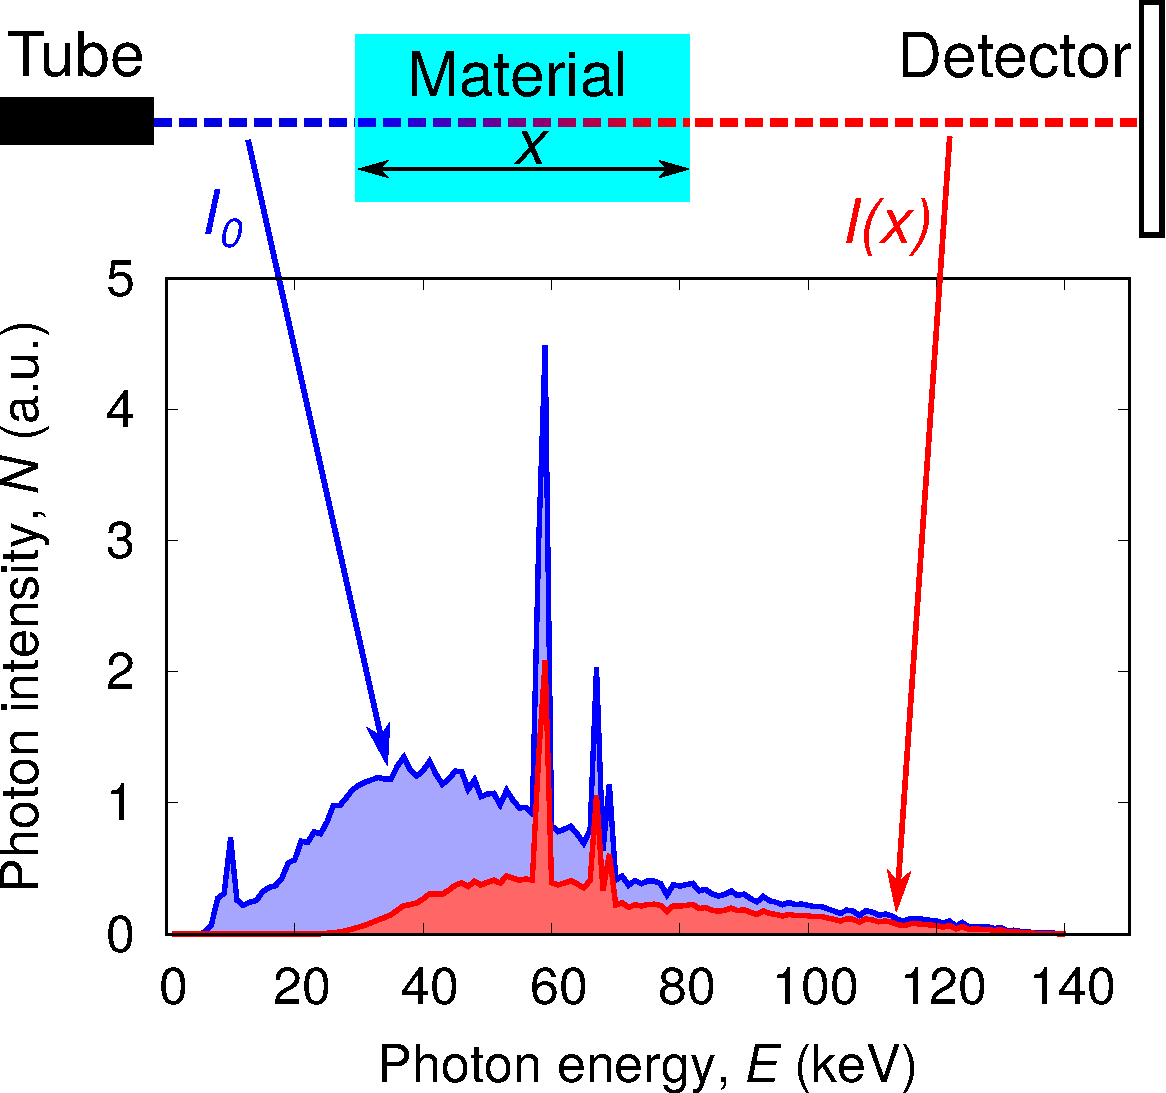
\includegraphics[width=\textwidth]
	{Sources/beam_hardening/x-ray_spectra_beam_hardening.pdf}}
\end{textblock}

\begin{textblock}{0.17}(0.5,0.02)
	\only<1>{
	\fbox{
	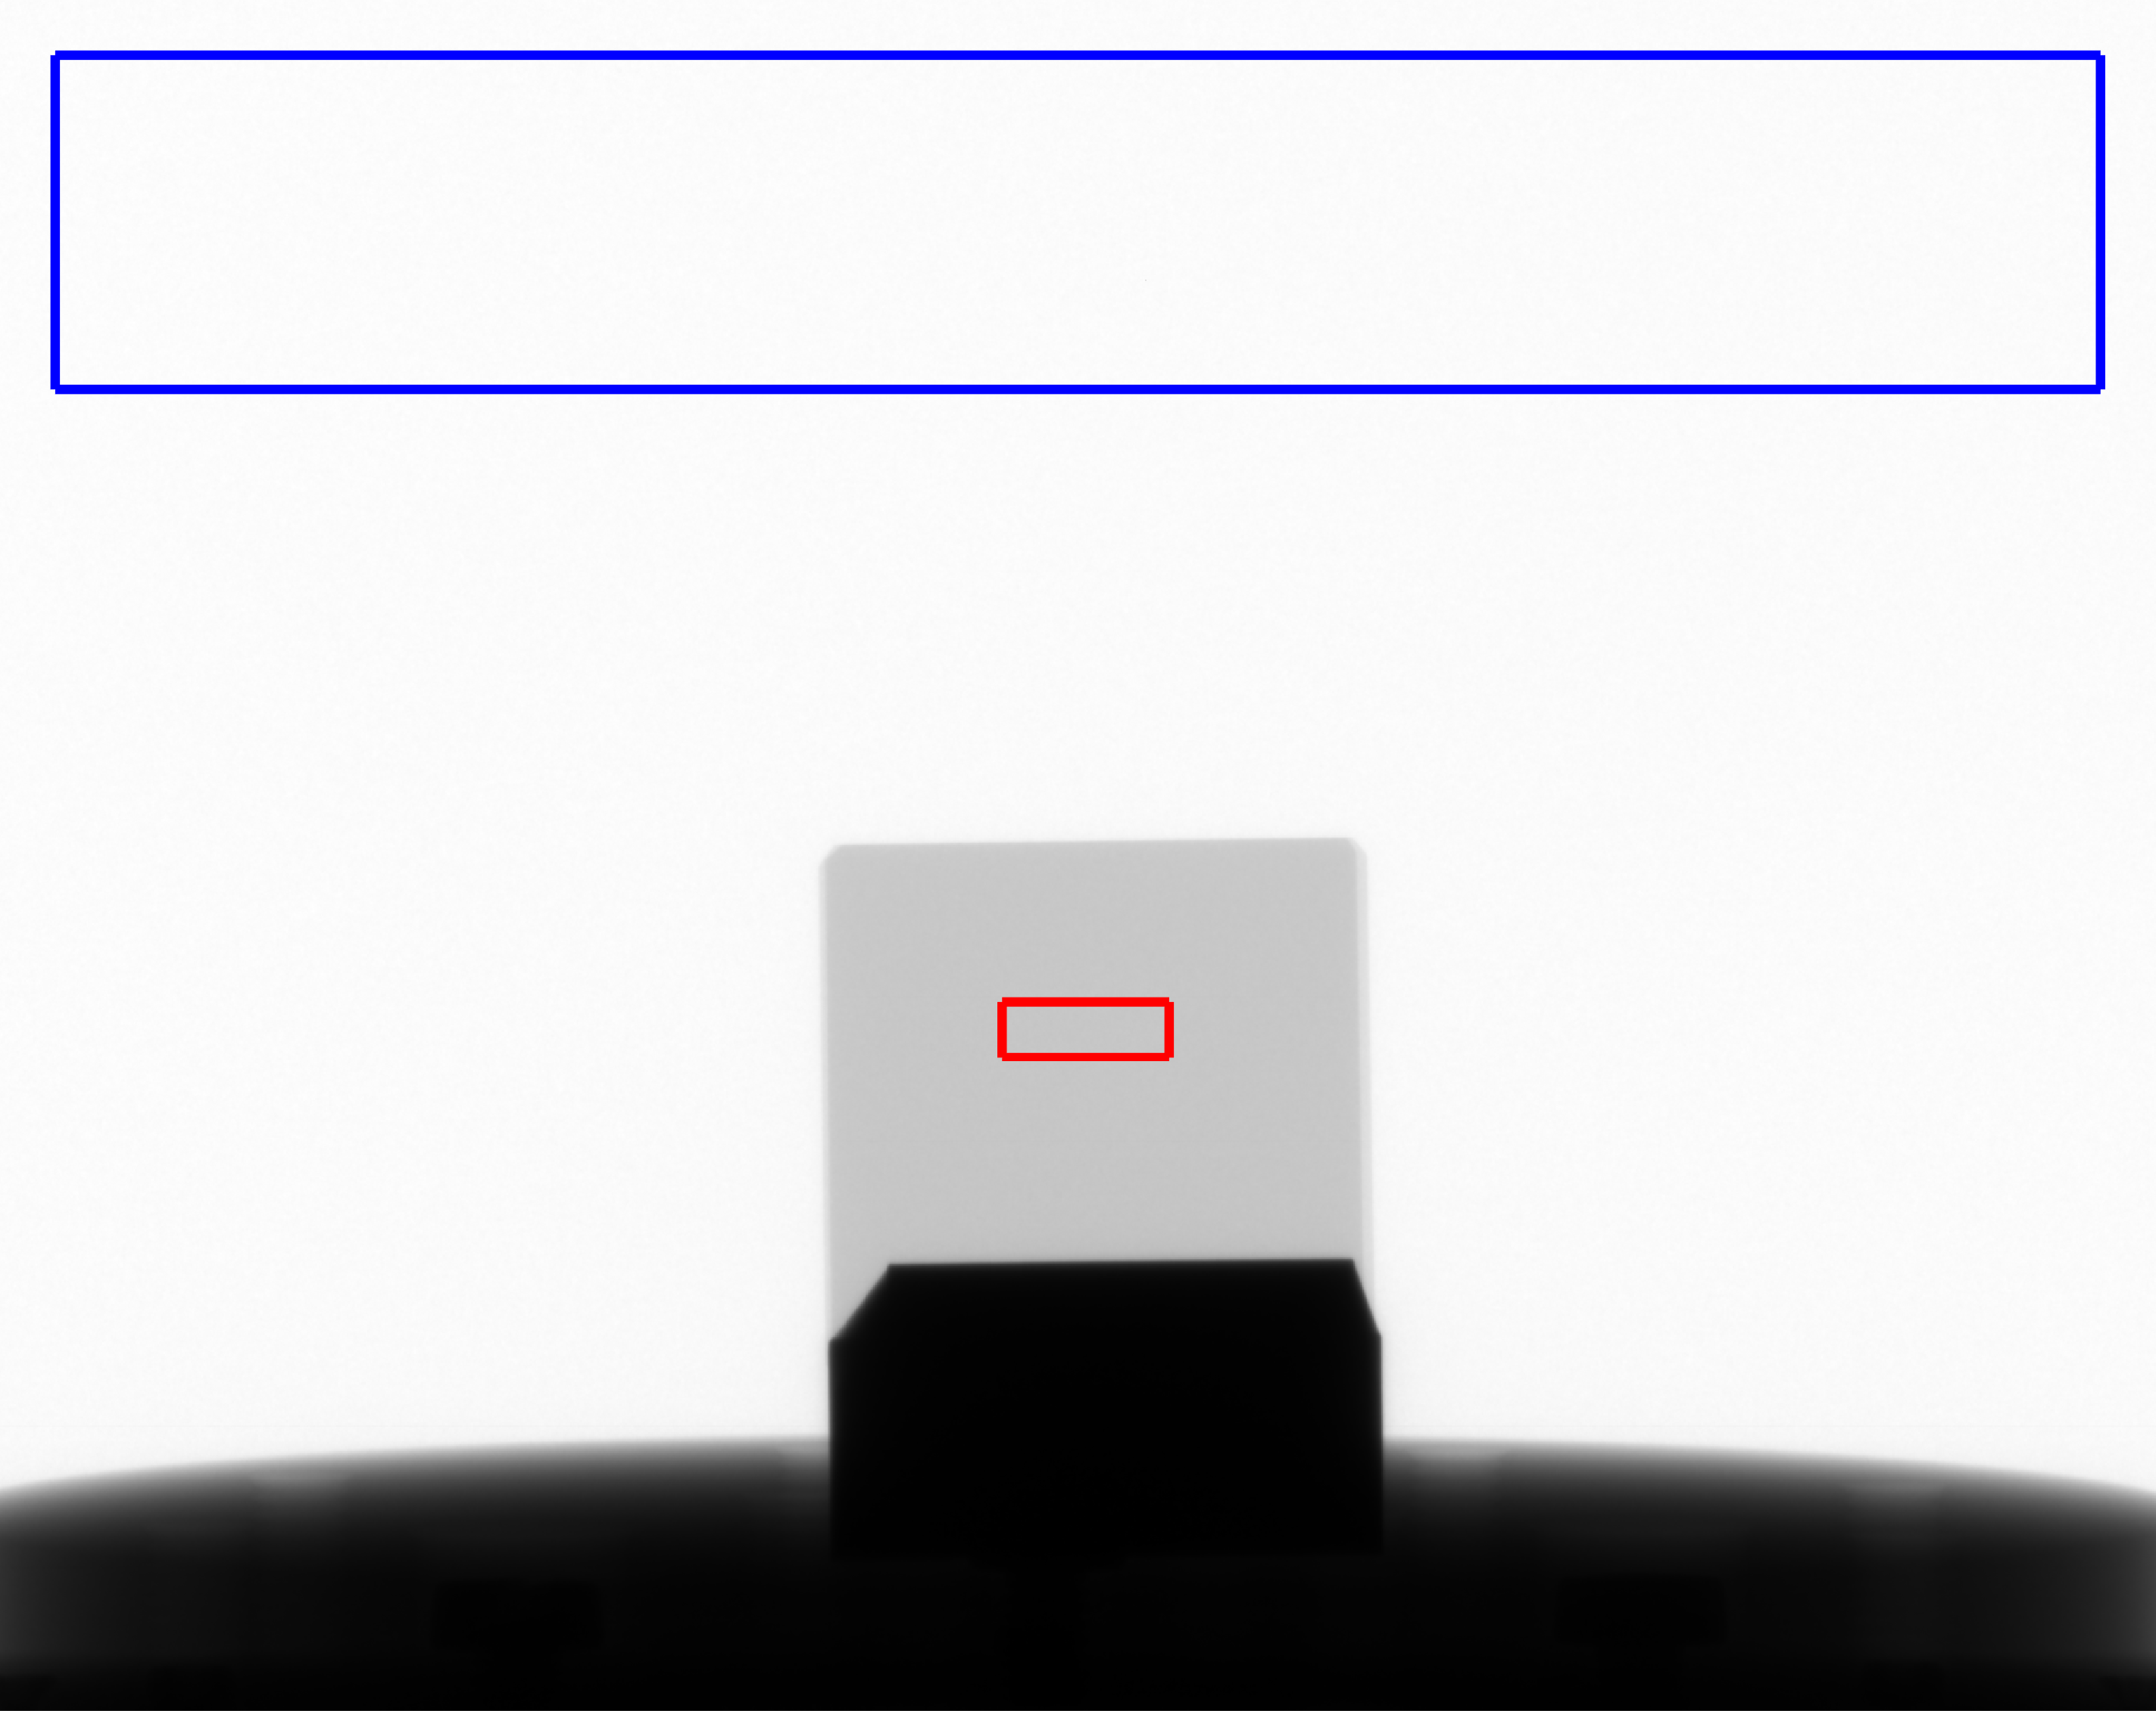
\includegraphics[width=\textwidth]
	{Sources/beam_hardening/02_plates.png}}}
	\only<2>{
	\fbox{
	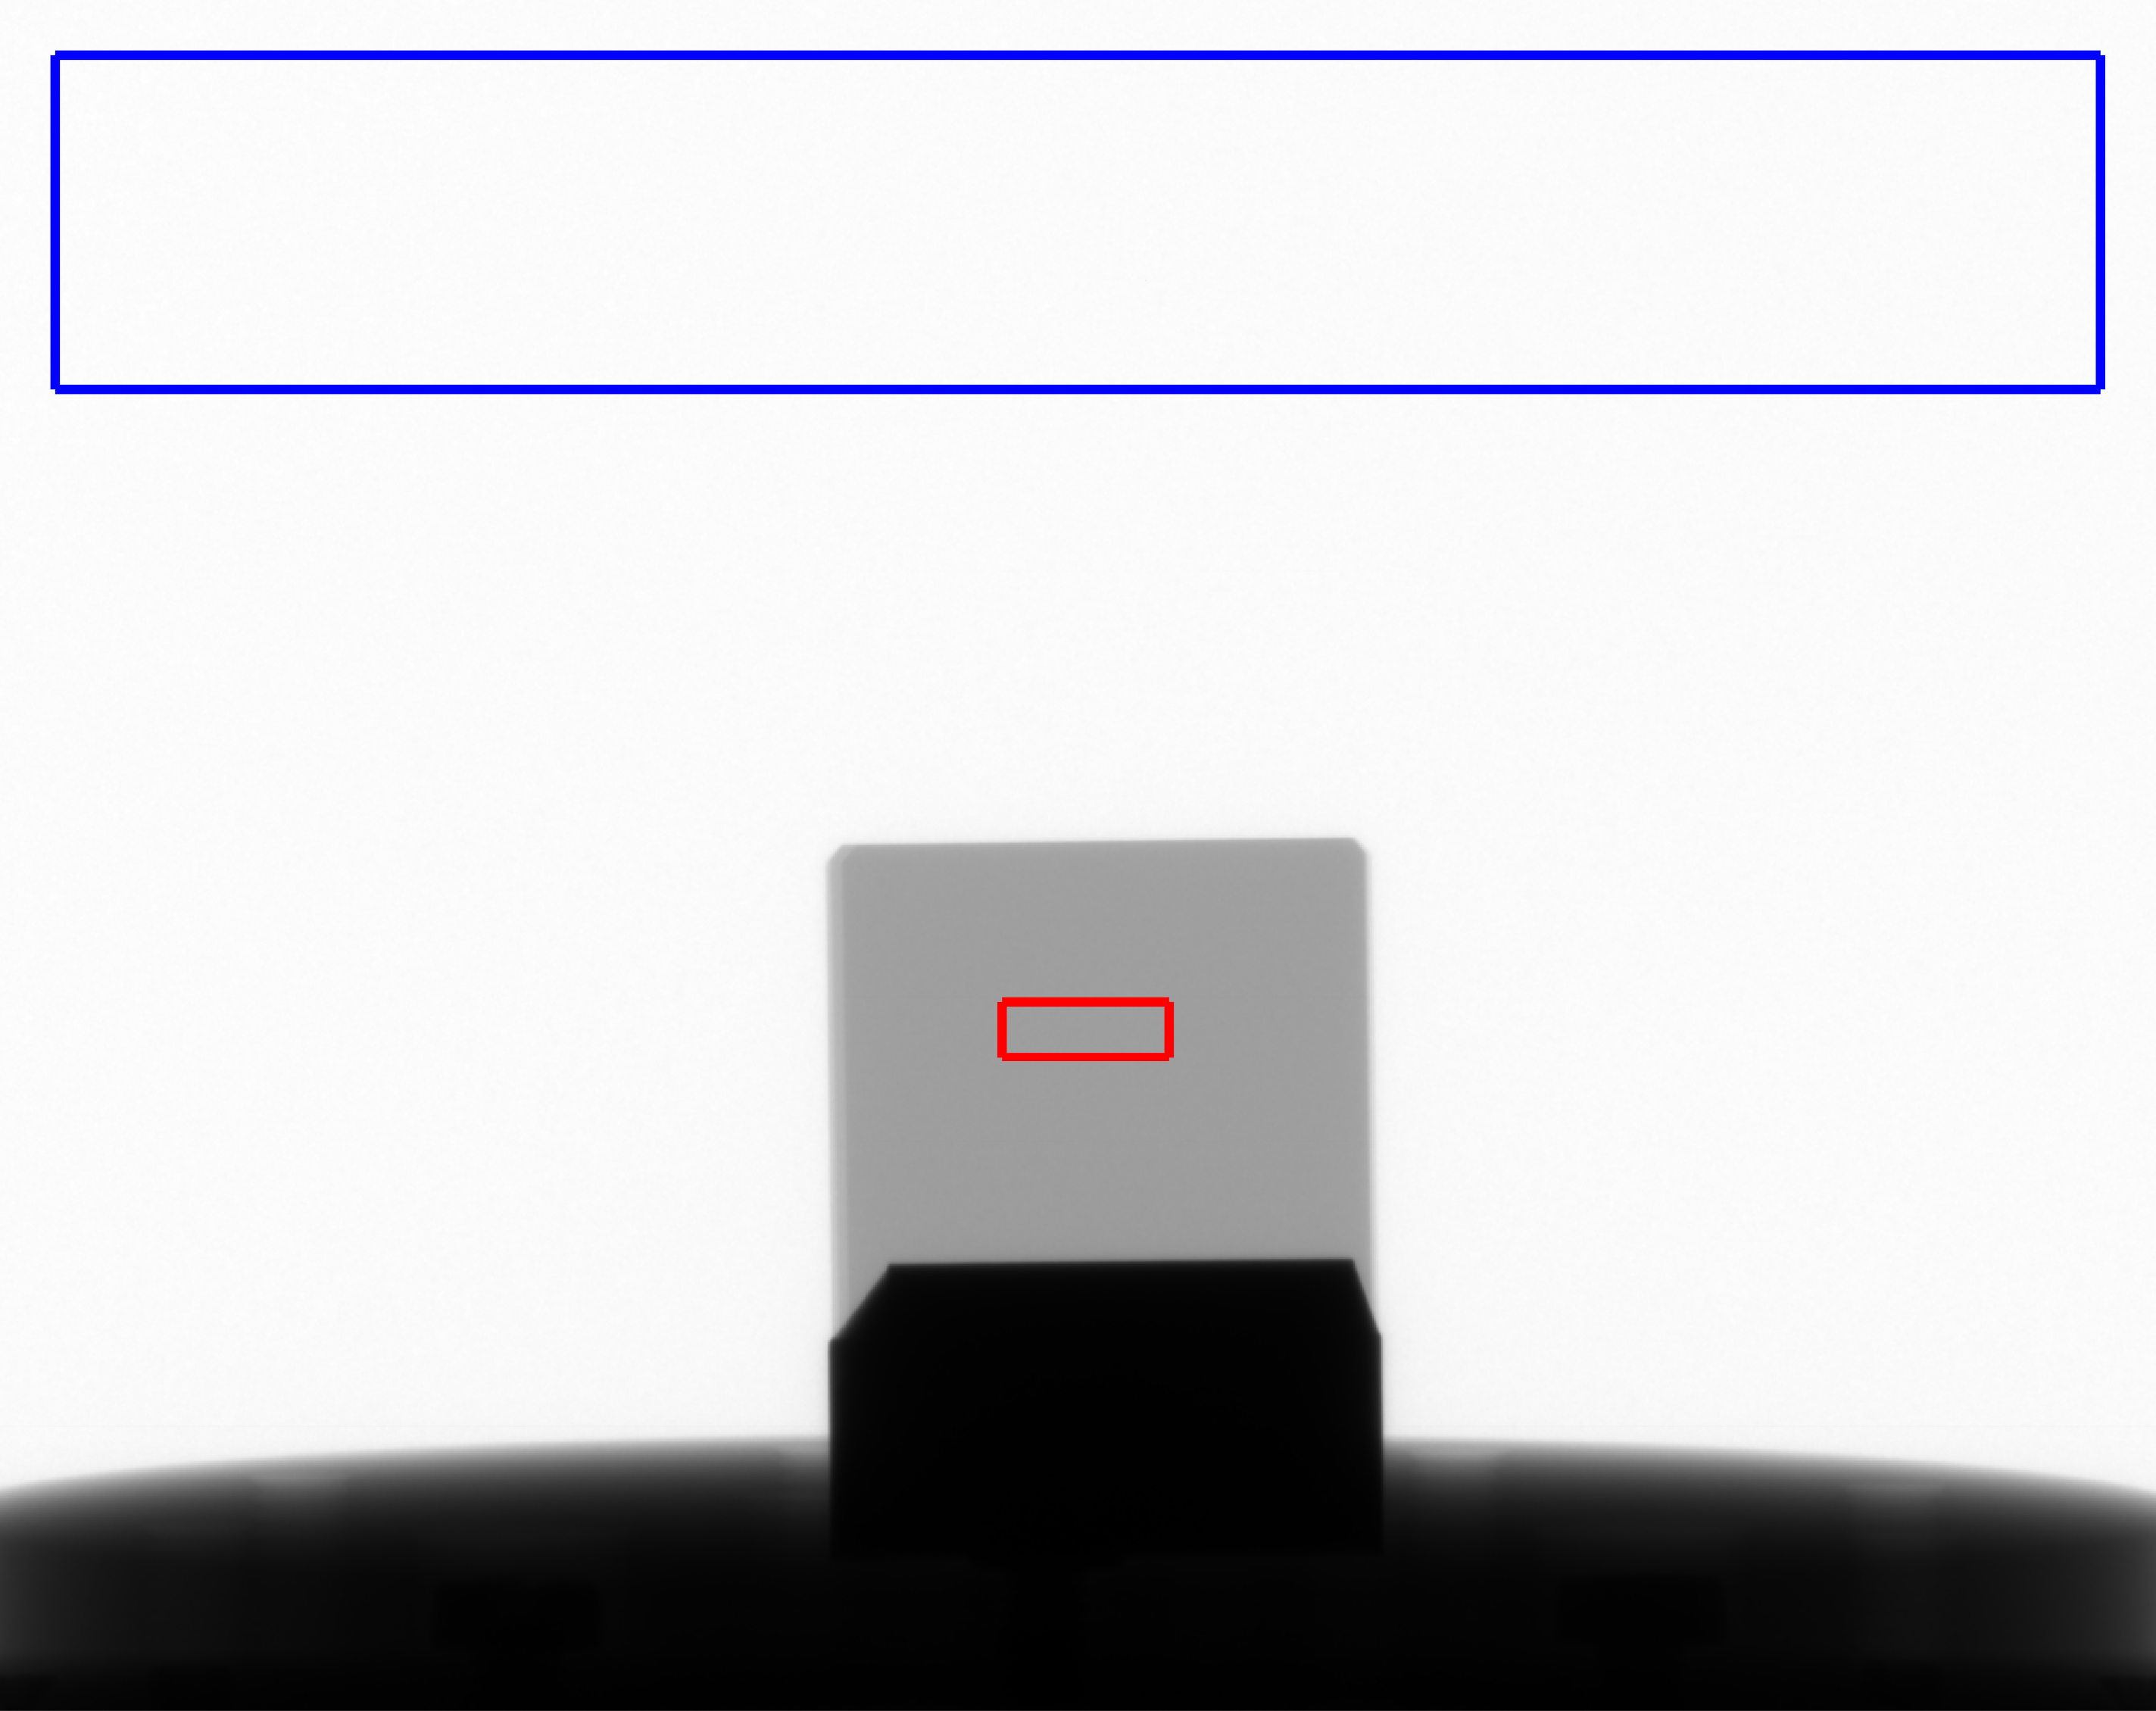
\includegraphics[width=\textwidth]
	{Sources/beam_hardening/04_plates.png}}}
	\only<3,4>{
	\fbox{
	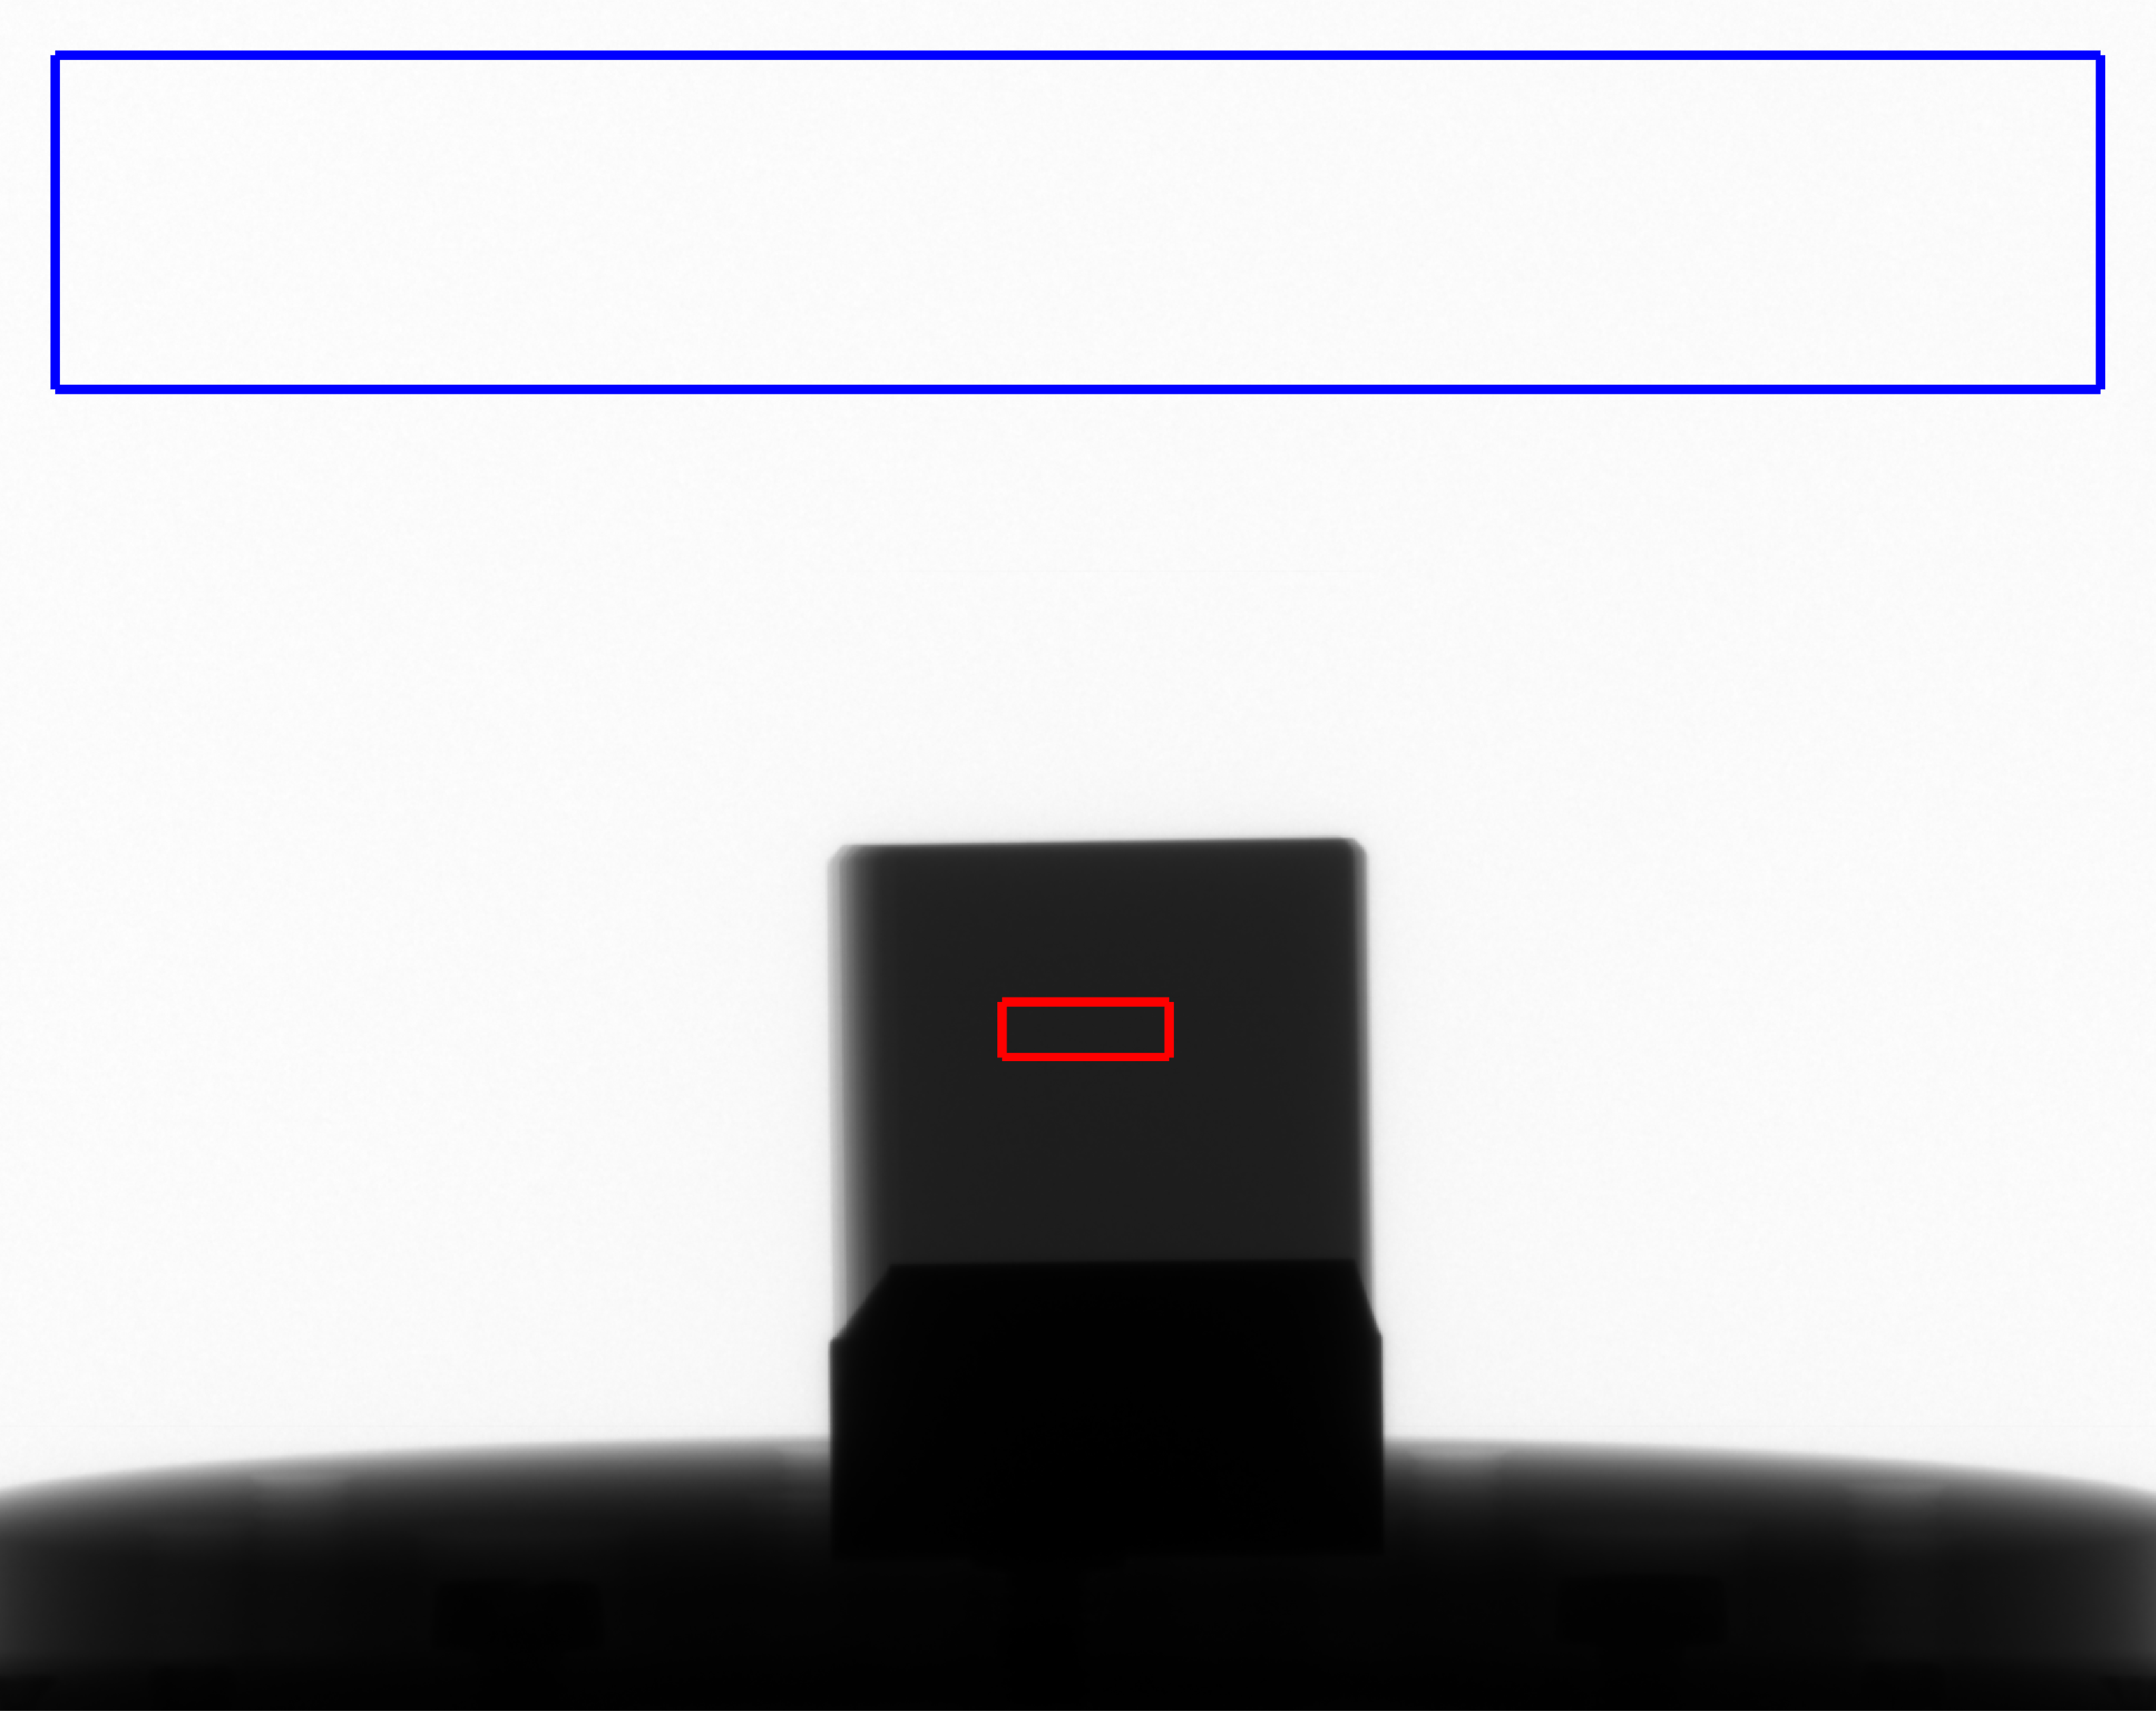
\includegraphics[width=\textwidth]
	{Sources/beam_hardening/20_plates.png}}}
\end{textblock}

\begin{textblock}{0.28}(0.7,0.05)
	\only<1,2,3>{
	\textcolor{darkgreen}{\textit{effective}} attenuation:
	\begin{align}
	\textcolor{red}{I(x)} &= 
	\textcolor{blue}{I_0} \exp(- \textcolor{darkgreen}{\mu_\text{eff}(x)}\, x) \nonumber
	\end{align}
	}
	\visible<4->{
	\textcolor{darkgreen}{\textit{effective}} attenuation:
	\begin{align}
	\textcolor{red}{I(x)} &= 
	\textcolor{blue}{I_0} 
	\exp(- \textcolor{darkgreen}{\mu_\text{eff}(x)}\, x) \nonumber\\
	\textcolor{darkgreen}{\mu_\text{eff} (x)} &= - 
	\frac{1}{x} 
	\frac{\textcolor{red}{I(x)}}{\textcolor{blue}{I_0}} \nonumber
	\end{align}
	}
\end{textblock}


\begin{textblock}{0.48}(0.5,0.3)
	\visible<4->{
	\includegraphics[width=\textwidth]
	{Sources/beam_hardening/attenuation_boro_glass_140kV.pdf}}
\end{textblock}

\begin{textblock}{0.15}(0.8,0.4)
	\centering
	\visible<4->{
	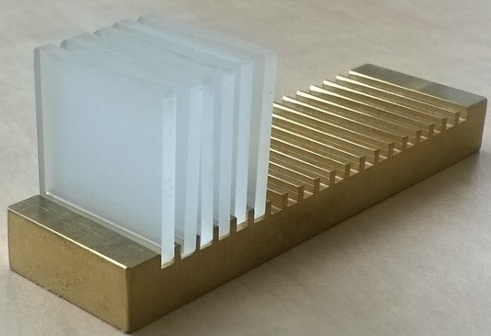
\includegraphics[width=\textwidth]
	{Sources/beam_hardening/plates_on_slide.png}}
\end{textblock}


}





%%%%%%%%%%%%%%%%%%%% Modeling mu_eff %%%%%%%%%%%%%%%%%%%%%%%%%%%%
\frame{
\begin{tikzpicture}[remember picture,overlay]
\fill[blue1]
(current page.north west) rectangle ([xshift=0.29\textwidth,yshift=0.33\textheight]current page.west|-{pic cs:end});
\end{tikzpicture}

\begin{textblock}{0.3}(0.02,0.03)
	\textcolor{white}{
		\Large Modeling of $\mu_\text{eff}(x)$}
\end{textblock}



\begin{textblock}{1.}(0.0,0.03)
	\centering
	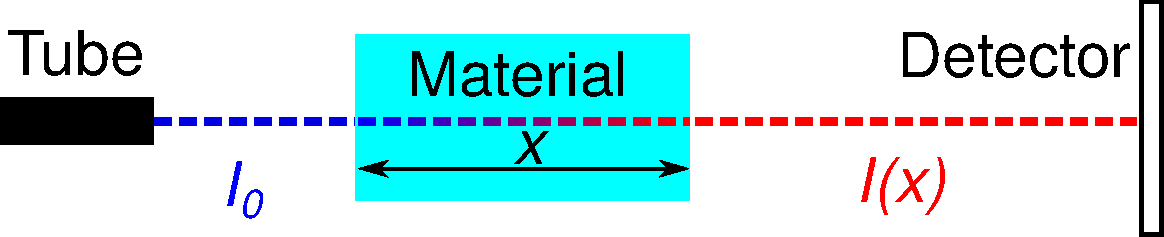
\includegraphics[width=0.4\textwidth]
	{Sources/beam_hardening/beam_through_material.pdf}
\end{textblock}

%% Photon spectrum
\begin{textblock}{0.32}(0.03,0.18)
	\centering
	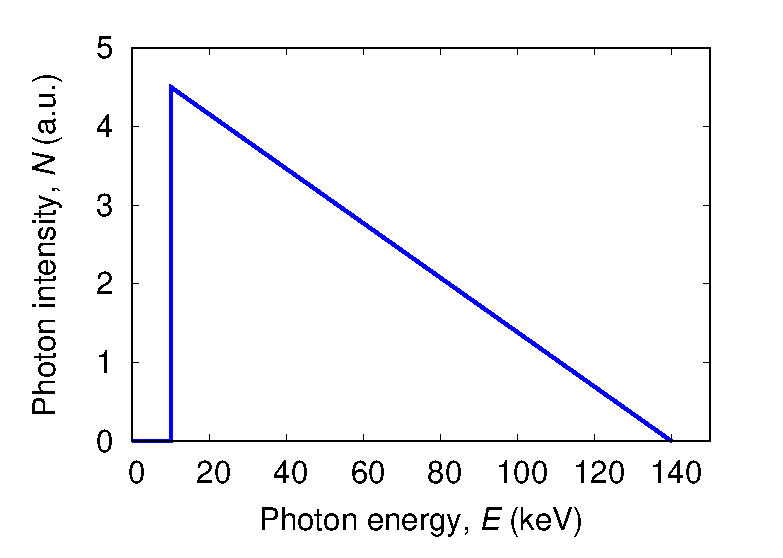
\includegraphics[width=\textwidth]
	{Sources/beam_hardening/linear_spectrum.eps}
\end{textblock}

\begin{textblock}{0.32}(0.03,0.17)
	\centering
	\hspace{0.5cm}
	\pgfsetfillopacity{1}\colorbox{blue1}{\pgfsetfillopacity{1}\textcolor{white}{
			$N (E) = -a E + b$}}
\end{textblock}

%% attenuation data
\begin{textblock}{0.32}(0.345,0.18)
	\centering
	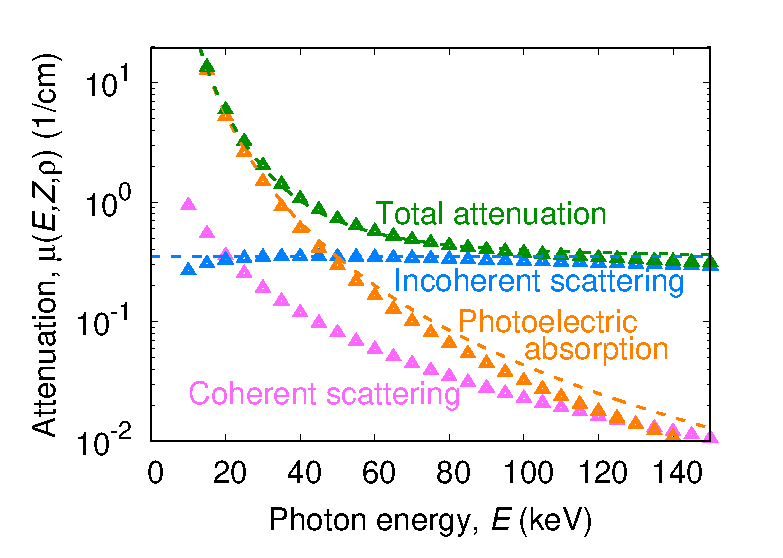
\includegraphics[width=\textwidth]
	{Sources/beam_hardening/XCOM_attenuation.eps}
\end{textblock}

\begin{textblock}{0.32}(0.345,0.17)
	\centering
	\hspace{0.5cm}
	\pgfsetfillopacity{1}\colorbox{darkgreen}{\pgfsetfillopacity{1}\textcolor{white}{
			$\mu (E) = \mu_\text{C} + c E^{-3}~\,^{(*)}$}}
\end{textblock}

%% detector curve
\begin{textblock}{0.32}(0.67,0.18)
	\centering
	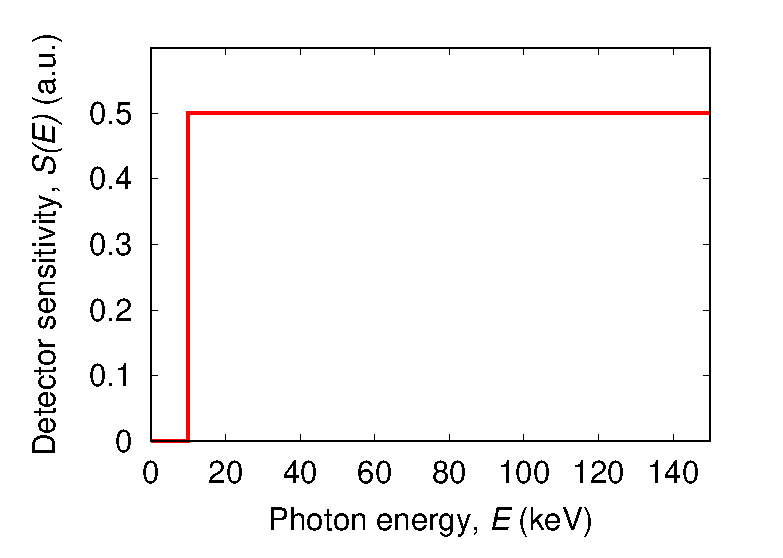
\includegraphics[width=\textwidth]
	{Sources/beam_hardening/detector_const.eps}
\end{textblock}

\begin{textblock}{0.32}(0.67,0.17)
	\centering
	\hspace{0.5cm}
	\pgfsetfillopacity{1}\colorbox{red}{\pgfsetfillopacity{1}\textcolor{white}{
		$S(E) = S~\Theta(E - E_\text{min})$}}
\end{textblock}

\begin{textblock}{0.5}(0.02,0.6)
	\only<1>{
		\begin{align}
		I(x) &\propto \int \textcolor{blue}{N(E)} \exp\{-
		\textcolor{darkgreen}{\mu(E,Z,\rho)} x\} 
		\textcolor{red}{S(E)}~\mathsf{d}E \nonumber\\
		&\textcolor{white}{\propto S \int_{E_\text{min}}^{E_\text{max}}
		(-a E + b) 
		\exp[-(\mu_\text{C} + c E^{-3}) x] 
		\mathsf{d}E}
		\nonumber
		\end{align}
	}
	\visible<2->{
		\begin{align}
		I(x) &\propto \int \textcolor{blue}{N(E)} \exp\{-
		\textcolor{darkgreen}{\mu(E,Z,\rho)} x\} 
		\textcolor{red}{S(E)}~\mathsf{d}E \nonumber \\
		&\propto \textcolor{red}{S} \int_{E_\text{min}}^{E_\text{max}}
		(\textcolor{blue}{-a E + b}) 
		\exp\{-(\textcolor{darkgreen}{\mu_\text{C} + c E^{-3}}) x\} 
		\mathsf{d}E 
		\nonumber
		\end{align}
	}
\end{textblock}



\begin{textblock}{0.32}(0.55,0.58)
	\visible<2->{
		\centering
		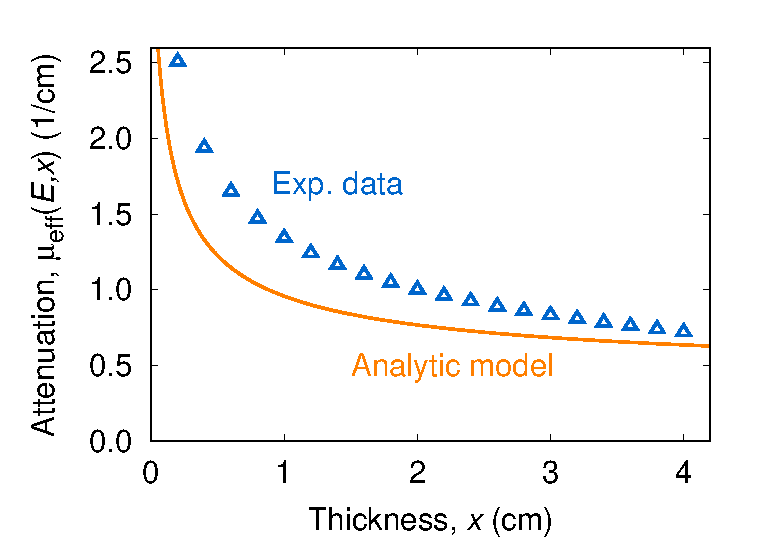
\includegraphics[width=\textwidth]
		{Sources/beam_hardening/attenuation_borosilicate_glass_voltages_first_principle_fit.eps}
	}
\end{textblock}

\begin{textblock}{0.9}(0.02,0.93)
	{\scriptsize
		$(*)$ XCOM supplied by NIST}
\end{textblock}

\begin{textblock}{1.}(0,0)
	\visible<3->{
		
\includegraphics[width=\textwidth]
		{Sources/beam_hardening/cross.pdf}}
\end{textblock}
}



%%%%%%%%%%%%%%%%%% Numerical approach %%%%%%%%%%%%%%%%%%%%%%%%%%%%
\frame{
\begin{tikzpicture}[remember picture,overlay]
\fill[blue1]
(current page.north west) rectangle ([xshift=0.28\textwidth,yshift=0.27\textheight]current page.west|-{pic cs:end});
\end{tikzpicture}

\begin{textblock}{0.23}(0.02,0.03)
	\centering
	\textcolor{white}{
	\Large Numerical approx.\ of 
	$\mu_\text{eff}(x)$}
\end{textblock}



\begin{textblock}{1.}(0.0,0.03)
	\centering
	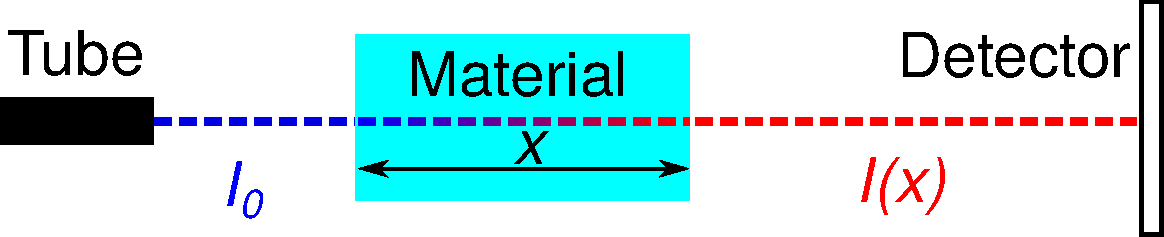
\includegraphics[width=0.4\textwidth]
	{Sources/beam_hardening/beam_through_material.pdf}
\end{textblock}

%% Photon spectrum
\begin{textblock}{0.32}(0.03,0.18)
	\centering
	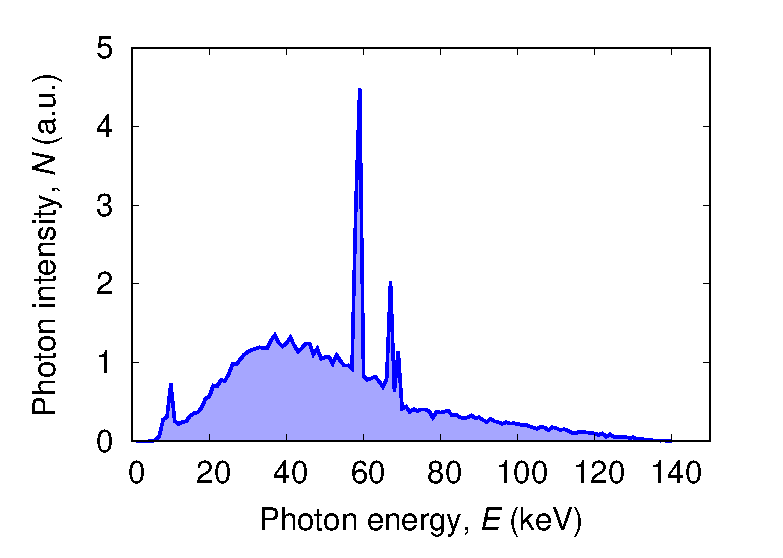
\includegraphics[width=\textwidth]
	{Sources/beam_hardening/N0_initial_spectrum_filled_curves.eps}
\end{textblock}

\begin{textblock}{0.32}(0.03,0.18)
	\centering
	\vspace{0.1cm}	
	\pgfsetfillopacity{0.85}\colorbox{blue1}{\pgfsetfillopacity{1}\textcolor{white}{
			Comet X-ray tube$^{(1)}$}}
\end{textblock}

%% attenuation data
\begin{textblock}{0.32}(0.345,0.18)
	\centering
	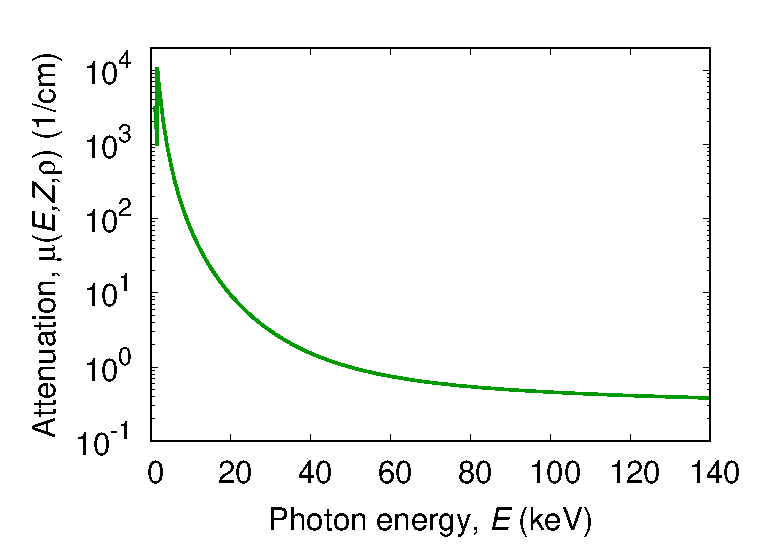
\includegraphics[width=\textwidth]
	{Sources/beam_hardening/Attenuation_vs_energy_Al.eps}
\end{textblock}

\begin{textblock}{0.32}(0.345,0.18)
	\centering
	\vspace{0.1cm}
	\pgfsetfillopacity{0.85}\colorbox{blue1}{\pgfsetfillopacity{1}\textcolor{white}{
			Aluminum$^{(2)}$}}
\end{textblock}

%% detector curve
\begin{textblock}{0.32}(0.67,0.18)
	\centering
		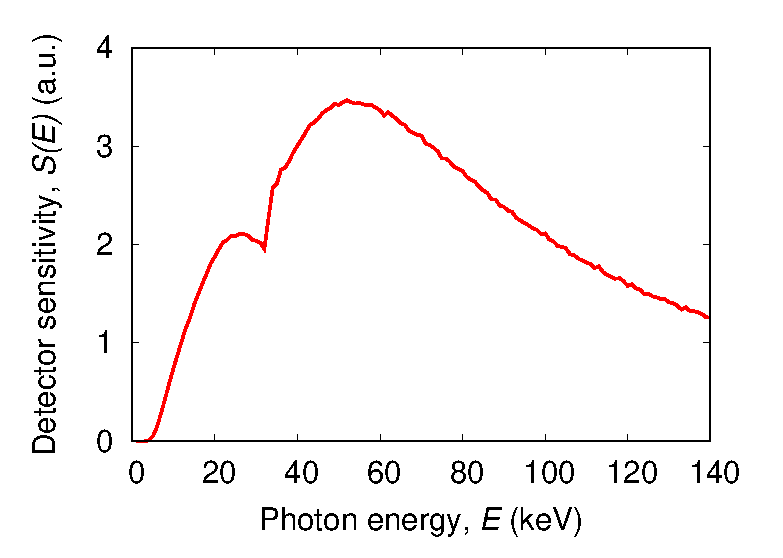
\includegraphics[width=\textwidth]
		{Sources/beam_hardening/Detector_response_0.eps}
\end{textblock}

\begin{textblock}{0.32}(0.67,0.18)
	\centering
	\vspace{0.1cm}
	\pgfsetfillopacity{0.85}\colorbox{blue1}{\pgfsetfillopacity{1}\textcolor{white}{
			XEye detector$^{(1)}$}}
\end{textblock}


\begin{textblock}{0.5}(0.02,0.6)
	\visible<1->{
	\begin{align}
		I(x) \propto &\int \textcolor{blue}{N(E)} \exp\{-
		\textcolor{darkgreen}{\mu(E,Z,\rho)} x\} 
		\textcolor{red}{S(E)}~\mathsf{d}E  \nonumber\\
		&\int \rightarrow \sum \nonumber
	\end{align}
}
\end{textblock}

\begin{textblock}{0.32}(0.55,0.58)
	\visible<2->{
	\centering
	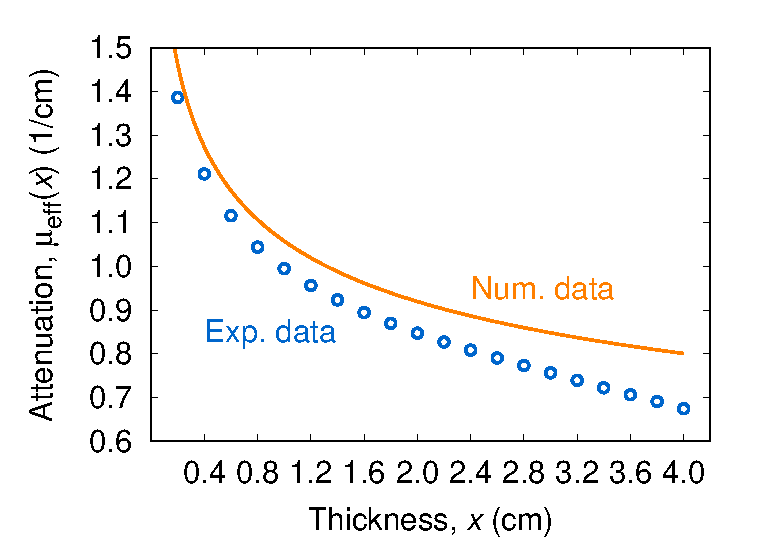
\includegraphics[width=\textwidth]
	{Sources/beam_hardening/mu_eff_140kV_exp_vs_numeric_data_norman.eps}
	}
\end{textblock}

\begin{textblock}{0.9}(0.02,0.9)
{\scriptsize
$(1)$ Supplied by Norman Uhlmann, Fraunhofer EZRT\\
$(2)$ XCOM supplied by NIST}
\end{textblock}

\begin{textblock}{1.}(0,0)
	\visible<3->{
	
\includegraphics[width=\textwidth]
{Sources/beam_hardening/cross.pdf}}
\end{textblock}
}




%% ------------- HEURISTIC MODEL-FUNCTION ------------
\frame{
\begin{tikzpicture}[remember picture,overlay]
\fill[blue1]
(current page.north west) rectangle ([xshift=0.52\textwidth,yshift=0.335\textheight]current page.west|-{pic cs:end});
\end{tikzpicture}

\begin{textblock}{0.5}(0.02,0.03)
	\textcolor{white}{
		\Large Heuristic model functions for $\mu_\text{eff}(x)$}
\end{textblock}

\begin{textblock}{0.39}(0.03,0.1)
	\only<1>{
	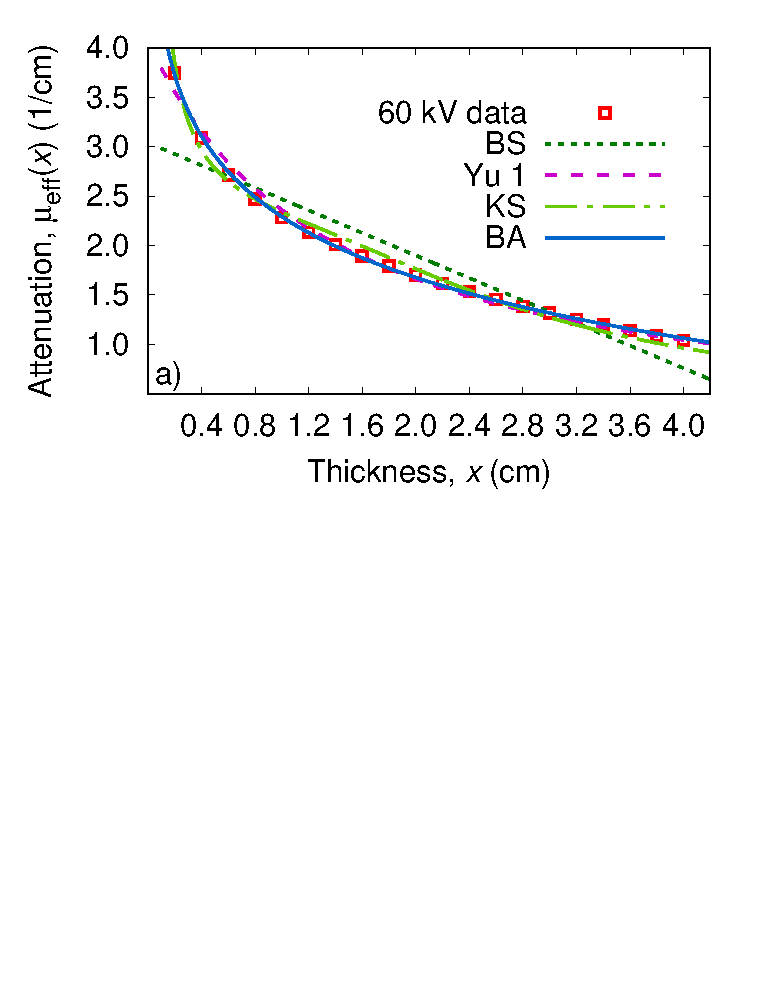
\includegraphics[width=\textwidth]
	{Sources/beam_hardening/borosilicate_glass_60kV_model_comparison_upper_plot0.eps}}
	\visible<2->{
	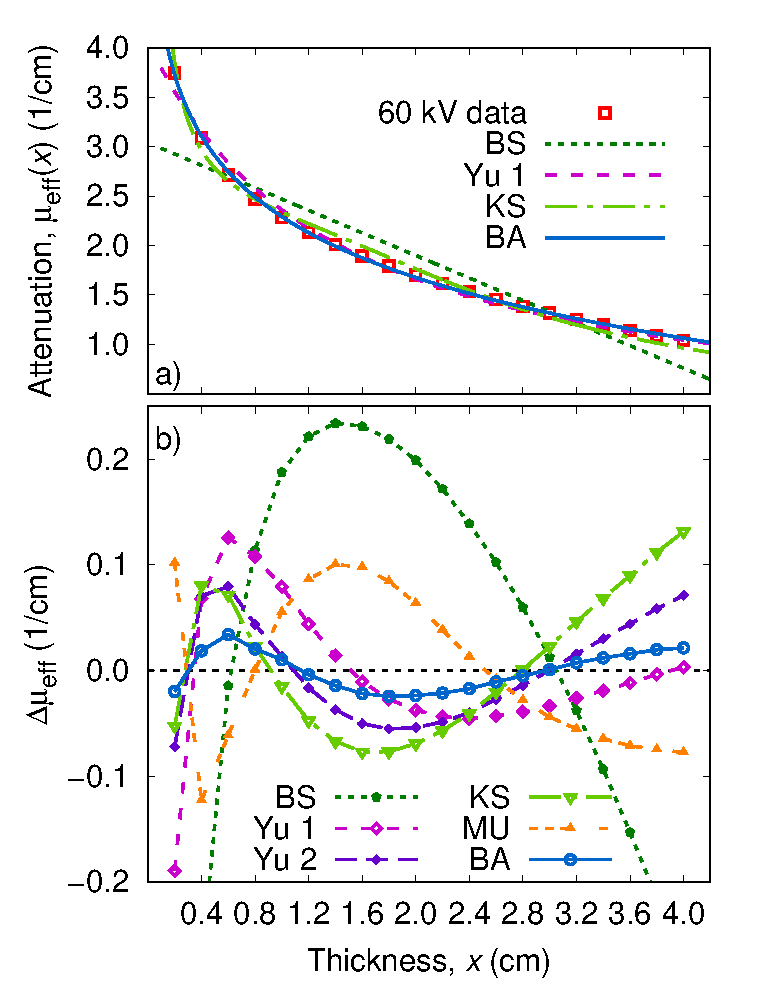
\includegraphics[width=\textwidth]
	{Sources/beam_hardening/borosilicate_glass_60kV_model_comparison_multiplot.eps}}
\end{textblock}


\begin{textblock}{0.5}(0.4, 0.12)
\only<1>{
	\begin{tabular}{ll}
		{\small
			\textcolor{BS}{$\mu_\text{eff} (x)= \mu_0 - \lambda x$}} &
		{\small Bjärngard \& Shackford} \\
		& {\small (1994)}\\[0.7cm]
		
		{\small	
			\textcolor{Yu1}{$\mu_\text{eff}(x) = \frac{\mu_0}{1+\lambda x}$}} &
		\multirow{2}{\linewidth}{\small Yu \textit{et al.} (1997)}\\
		
		{\small
			\textcolor{white}{$\mu_\text{eff}(x) = \frac{\mu_0}{(1+\lambda x)^\beta}$}} \\[0.7cm]
		
		{\small
			\textcolor{KS}{
				$\mu_\text{eff}(x) = \mu(E_\text{max}) +
				\frac{2 \mu_1}{x \sqrt{-\lambda_1^2 + 4 \lambda_2}} \times$}} & Kleinschmidt (1999)
		\\
		\multicolumn{2}{l}{\small
			\textcolor{KS}{
				$\quad\left[
				\arctan\left(
				\frac{\lambda_1 + 2 \lambda_2 x}{\sqrt{-\lambda_1^2 + 4 \lambda_2}}
				\right)
				-\arctan\left(
				\frac{\lambda_1}{\sqrt{-\lambda_1^2 + 4 \lambda_2}}
				\right)
				\right]
				$ }} \\[0.7cm]
		
		{\small
			\textcolor{white}{$\mu_\text{eff}(x) = -\frac{1}{x} \ln \left[A+B \exp(-x/C)\right]$}} & 
		{\small
			\textcolor{white}{
			Mudde \textit{et al.} (2008) }}\\[0.7cm]
		
		{\small
			\textcolor{BA}{$\boldsymbol{\mu_\text{eff}(x) = a + \frac{b}{x^\alpha}}$}} &
		{\small \textbf{Baur \textit{et al.} (2019)}}\\
		& {\small (this work)}
	\end{tabular}
}
	
\visible<2->{
\begin{tabular}{ll}
{\small
	\textcolor{BS}{$\mu_\text{eff} (x)= \mu_0 - \lambda x$}} &
	{\small Bjärngard \& Shackford} \\
		& {\small (1994)}\\[0.7cm]
	
{\small	
\textcolor{Yu1}{$\mu_\text{eff}(x) = \frac{\mu_0}{1+\lambda x}$}} &
\multirow{2}{\linewidth}{\small Yu \textit{et al.} (1997)}\\

{\small
\textcolor{Yu2}{$\mu_\text{eff}(x) = \frac{\mu_0}{(1+\lambda x)^\beta}$}} \\[0.7cm]

{\small
\textcolor{KS}{
	$\mu_\text{eff}(x) = \mu(E_\text{max}) +
	\frac{2 \mu_1}{x \sqrt{-\lambda_1^2 + 4 \lambda_2}} \times$}} & Kleinschmidt (1999)
\\
\multicolumn{2}{l}{\small
\textcolor{KS}{
	$\quad\left[
	\arctan\left(
	\frac{\lambda_1 + 2 \lambda_2 x}{\sqrt{-\lambda_1^2 + 4 \lambda_2}}
	\right)
	-\arctan\left(
	\frac{\lambda_1}{\sqrt{-\lambda_1^2 + 4 \lambda_2}}
	\right)
	\right]
	$ }} \\[0.7cm]

{\small
\textcolor{MU}{$\mu_\text{eff}(x) = -\frac{1}{x} \ln \left[A+B \exp(-x/C)\right]$}} & 
{\small
	Mudde \textit{et al.} (2008) }\\[0.7cm]

{\small
\colorbox{BA}{\textcolor{white}{$\boldsymbol{\mu_\text{eff}(x) = a + \frac{b}{x^\alpha}}$}}} &
{\small \textbf{Baur \textit{et al.} (2019)}}\\
& {\small (this work)}
\end{tabular}
}
\end{textblock}
}

%% ------------- RESULTS -----------------------------
\frame{
\begin{tikzpicture}[remember picture,overlay]
\fill[blue1]
(current page.north west) rectangle ([xshift=0.22\textwidth,yshift=-10.cm]current page.west|-{pic cs:end});
\end{tikzpicture}

\begin{textblock}{0.2}(0.01,0.15)
	\textcolor{white}{\Large
	{Universality of }{\large$\boldsymbol{\mu_\text{eff}(x) = a + \frac{b}{x^\alpha}}$}}
\end{textblock}

\begin{textblock}{0.2}(0.005,0.35)
	\centering
	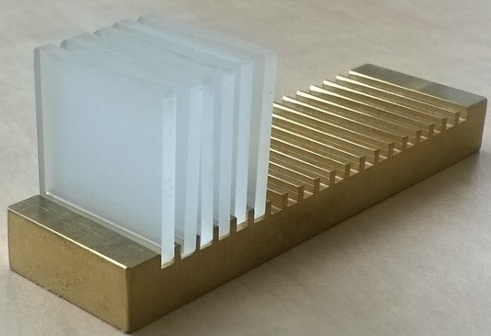
\includegraphics[width=0.8\textwidth]
	{Sources/beam_hardening/plates_on_slide.png}
\end{textblock}

\begin{textblock}{0.2}(0.005,0.65)
	\centering
	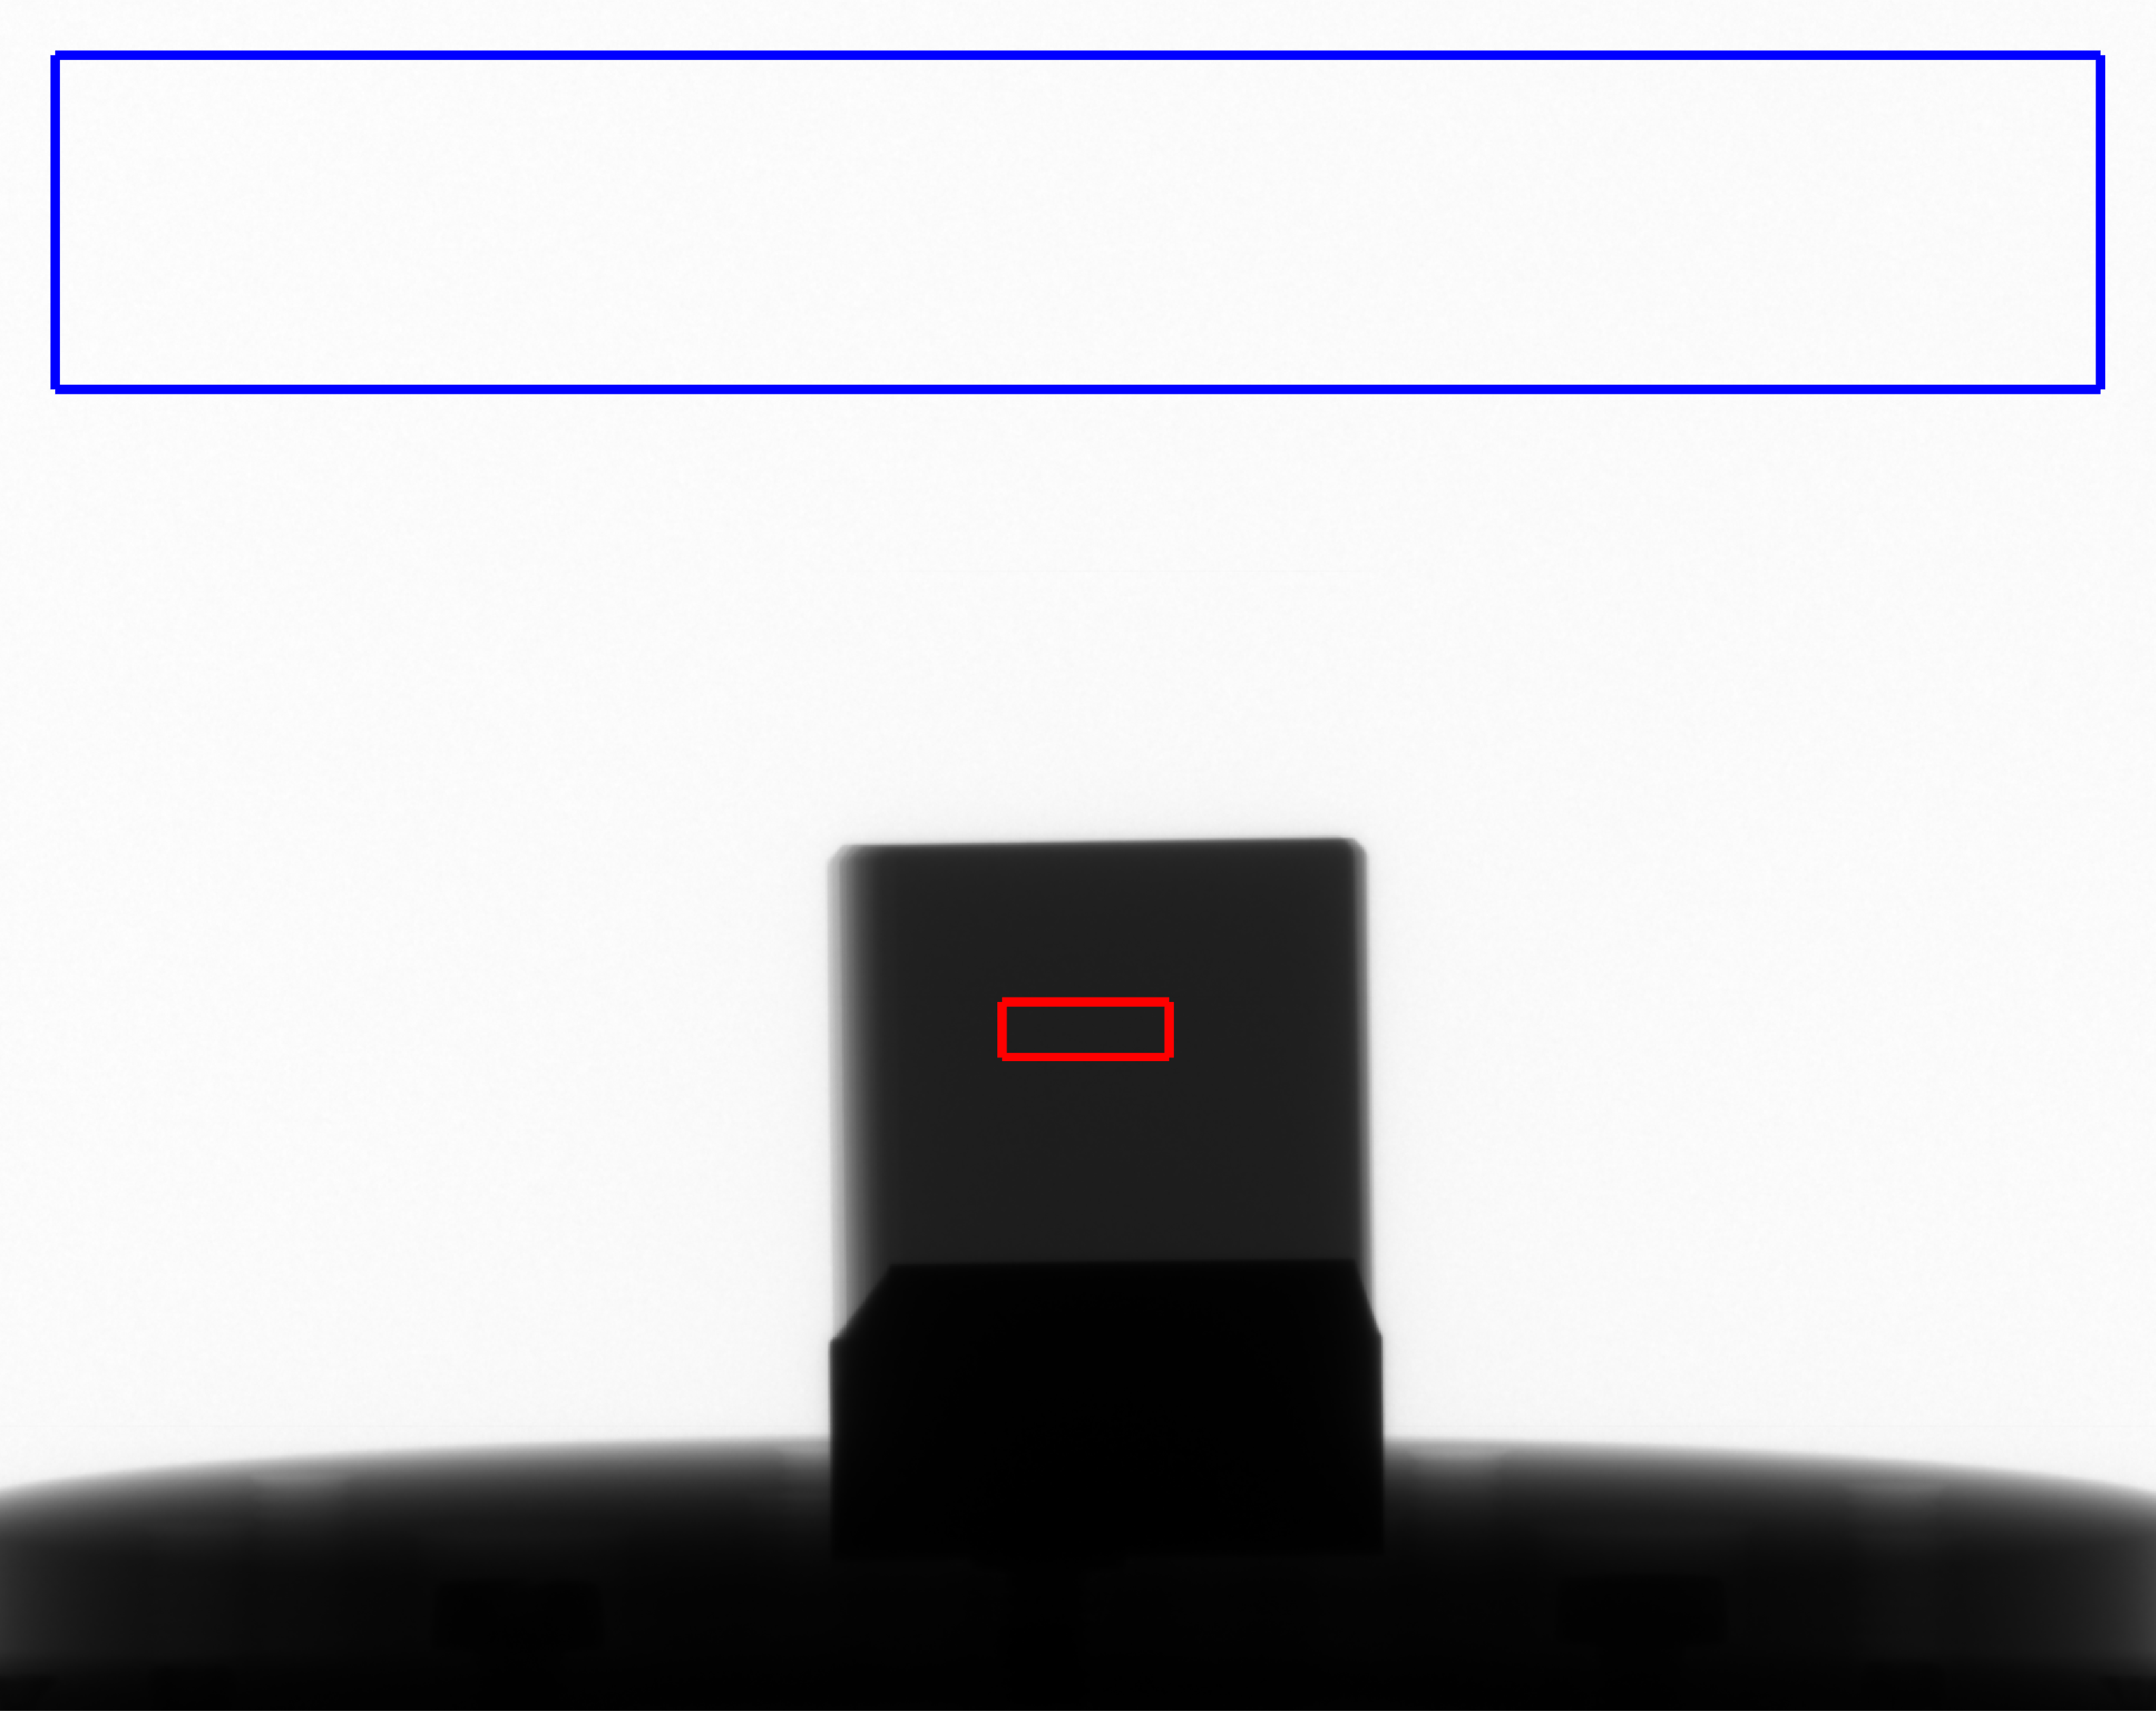
\includegraphics[width=0.8\textwidth]
	{Sources/beam_hardening/20_plates.png}
\end{textblock}



%%% VOLTAGES
\begin{textblock}{0.39}(0.23,0.0)
	\visible<1->{
		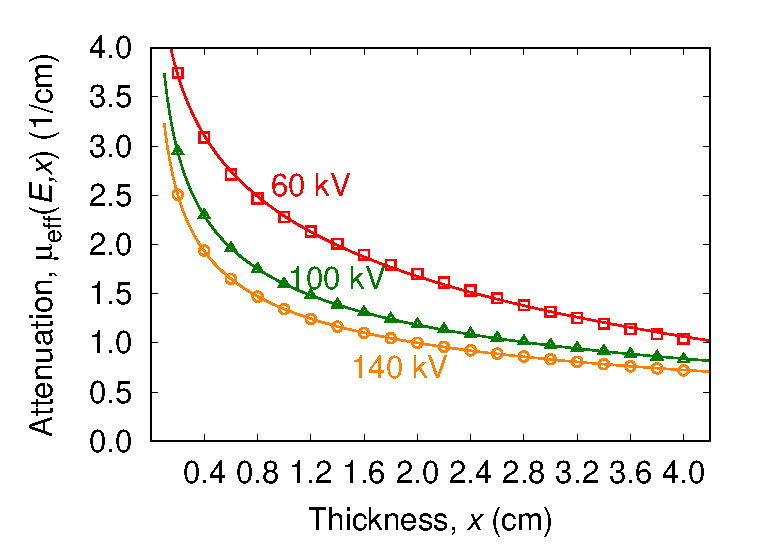
\includegraphics[width=\textwidth]
		{Sources/beam_hardening/borosilicate_glass_voltages_mu_eff.eps}}
\end{textblock}

\begin{textblock}{0.6}(0.23,0.0)
	\vspace{0.5cm}	
	\visible<1->{
		\hspace{3.cm} \colorbox{blue1}{\textcolor{white}{
		 varying voltages}}}
\end{textblock}


%% FILTERS
\begin{textblock}{0.39}(0.62,0.0)
	\visible<2->{
		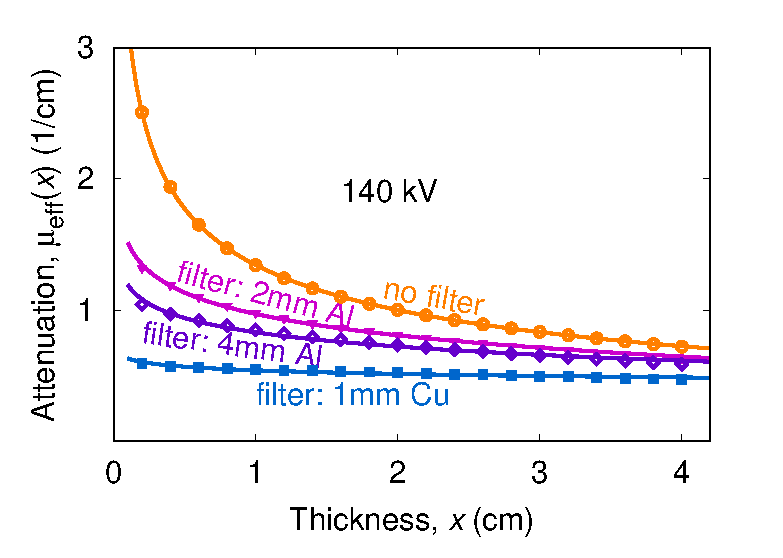
\includegraphics[width=\textwidth]
		{Sources/beam_hardening/borosilicate_glass_filters_mu_eff.eps}}
\end{textblock}

\begin{textblock}{0.6}(0.62,0.0)
	\vspace{0.5cm}	
	\visible<2->{
		\hspace{3.cm} \colorbox{blue1}{\textcolor{white}{
				different filters}}}
\end{textblock}

%% MATERIALS
\begin{textblock}{0.39}(0.23,0.5)
	\visible<3->{
		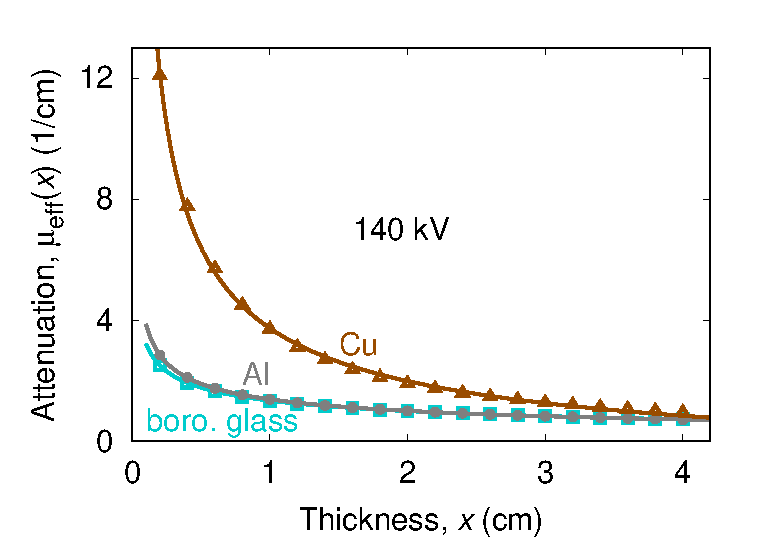
\includegraphics[width=\textwidth]
		{Sources/beam_hardening/materials_mu_eff_140kV_fit.eps}}
\end{textblock}

\begin{textblock}{0.6}(0.23,0.5)
	\vspace{0.5cm}	
	\visible<3->{
		\hspace{3.cm} \colorbox{blue1}{\textcolor{white}{
				different materials}}}
\end{textblock}

%% SETUPS
\begin{textblock}{0.39}(0.62,0.5)
	\visible<4->{
		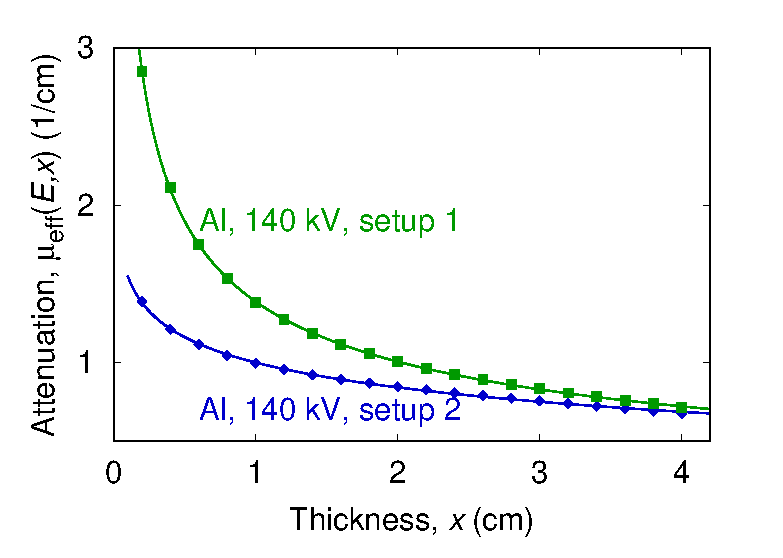
\includegraphics[width=\textwidth]
		{Sources/beam_hardening/comp_both_setups.eps}}
\end{textblock}

\begin{textblock}{0.6}(0.62,0.5)
	\vspace{0.5cm}	
	\visible<4->{
		\hspace{3.cm} \colorbox{blue1}{\textcolor{white}{
				2 X-ray setups}}}
\end{textblock}
}

%% ------------- MATERIAL THICKNESS X
\frame{
\begin{tikzpicture}[remember picture,overlay]
\fill[blue1]
(current page.north west) rectangle ([xshift=0.55\textwidth,yshift=0.34\textheight]current page.west|-{pic cs:end});
\end{tikzpicture}

\begin{textblock}{0.5}(0.02,0.03)
	\textcolor{white}{
		\Large Determining the material thickness $x$}
\end{textblock}


\begin{textblock}{0.5}(0.05,0.15)
\visible<1->{
Generalized Beer-Lambert
\[ I(x) = I_0 \exp(-\mu_\text{eff} (x) \, x) \]

Model function
\[ \mu_\text{eff} (x) = a + \frac{b}{x^\alpha} \]\\[0.5cm]
}

\visible<2->{
Solve
\[ a x + b x^{1-\alpha} + \ln \left(\frac{I(x)}{I_0}\right) = 0\]
e.g.\ Newton's method or look-up table}
\end{textblock}

\begin{textblock}{0.4}(0.55,0.05)
\only<1>{
	\includegraphics[width=\textwidth]
	{Sources/beam_hardening/borosilicate_glass_mueff_3datapoints_multiplot_1.eps}
}

\only<2>{
	\includegraphics[width=\textwidth]
	{Sources/beam_hardening/borosilicate_glass_mueff_3datapoints_multiplot_2.eps}
}

\visible<3->{
	\includegraphics[width=\textwidth]
	{Sources/beam_hardening/borosilicate_glass_mueff_3datapoints_multiplot.eps}
}
\end{textblock}
}

%% ------------- Applications ------------------------
\frame{
\begin{tikzpicture}[remember picture,overlay]
\fill[blue1]
(current page.north west) rectangle ([xshift=1.\paperwidth,yshift=0.33\paperheight]current page.west|-{pic cs:end});
\end{tikzpicture}

\begin{textblock}{1.}(0.02,0.03)
	\textcolor{white}{
		\Large Migrating shear bands in shaken granular matter, Kollmer \textit{et al} (2020)}
\end{textblock}

\begin{textblock}{0.9}(0.05,0.12)
	\centering
	\only<1>{
	\includegraphics[width=0.8\textwidth]
	{Sources/beam_hardening/migrating_shearband.pdf}}
\end{textblock}
}

\frame{
	\begin{tikzpicture}[remember picture,overlay]
	\fill[blue1]
	(current page.north west) rectangle ([xshift=12.cm,yshift=-10.cm]current page.east|-{pic cs:end});
	\end{tikzpicture}
	\begin{textblock}{0.9}(0.05,0.15)
		\centering
			{\huge
			\textcolor{white}{
			Measuring granular dynamics with}}\\[0.2cm]
		{\Huge
			\textcolor{white}{
			X-ray Digital Fourier Analysis (X-DFA)}}
	\end{textblock}

	\begin{textblock}{0.9}(0.05,0.45)
		\centering
		\movie[width =0.25\textwidth, poster, loop]
		{\includegraphics[width=0.25\textwidth]{Sources/X-DFA/cropped_80kV_340uA_38ms_0000.png}}
		{Sources/X-DFA/3500mul_per_min_cropped_roi_512x512.avi}
	\end{textblock}
	
	\begin{textblock}{0.9}(0.05,0.93)
		\centering
		{
		\textcolor{white}{
		In collaboration with M.\ Escobedo \& S.\ Egelhaaf, University of Düsseldorf}}
	\end{textblock}
}


\frame{
\begin{tikzpicture}[remember picture,overlay]
\fill[blue1]
(current page.north west) rectangle ([xshift=0.5\paperwidth,yshift=0.33\paperheight]current page.west|-{pic cs:end});
\end{tikzpicture}

\begin{textblock}{0.6}(0.02,0.03)
	\textcolor{white}{
		\Large The system: A liquid fluidized bed}
\end{textblock}

\begin{textblock}{0.6}(0.03,0.12)
	\visible<1->{
	\includegraphics[width=\textwidth]{Sources/X-DFA/experiment-fluidized_bed_1.pdf}}
\end{textblock}

\begin{textblock}{0.6}(0.4,0.9)
	$0.45 < \Phi < 0.56$
\end{textblock}


\begin{textblock}{0.3}(0.65,0.1)
	\centering
	\only<1>{
		Radiogram\\
		\includegraphics[width=\textwidth]{Sources/X-DFA/radiogram.png}}
\end{textblock}		

\begin{textblock}{0.3}(0.65,0.05)
	\visible<2->{
	\centering
	Particle tracking}
\end{textblock}

\begin{textblock}{0.3}(0.65,0.1)
	\visible<2->{
	\movie[width = \textwidth]
	{\includegraphics[width = \textwidth]{Sources/X-DFA/centroid_bronze_tracer_frame_nr_0000.png}}
	{Sources/X-DFA/centroid_bronze_tracer_4.mp4}}
\end{textblock}

\begin{textblock}{0.3}(0.65,0.1)
	\centering
	\visible<3->{\includegraphics[width=\textwidth]{Sources/X-DFA/cross.pdf}}
\end{textblock}
}

\begin{frame}[noframenumbering]
\begin{tikzpicture}[remember picture,overlay]
\fill[blue1]
(current page.north west) rectangle ([xshift=0.51\paperwidth,yshift=0.33\paperheight]current page.west|-{pic cs:end});
\end{tikzpicture}

\begin{textblock}{0.6}(0.02,0.03)
	\textcolor{white}{
		\Large The system: A liquid fluidized bed}
\end{textblock}

\begin{textblock}{0.6}(0.03,0.12)
		\includegraphics[width=\textwidth]{Sources/X-DFA/experiment-fluidized_bed_1.pdf}
\end{textblock}

\begin{textblock}{0.6}(0.42,0.9)
	$0.45 < \Phi < 0.56$
\end{textblock}


\begin{textblock}{0.3}(0.65,0.03)
	\centering
	Radiogram\\
		\includegraphics[width=\textwidth]{Sources/X-DFA/radiogram_ROI_marked.png}
\end{textblock}		

\begin{textblock}{0.3}(0.65,0.6)
	\centering
	\fbox{
	\movie[height=0.65\textwidth, poster]
	{\includegraphics[width=0.65\textwidth]{Sources/X-DFA/cropped_80kV_340uA_38ms_0000.png}}
	{Sources/X-DFA/3500mul_per_min_cropped_roi_512x512.avi}
	}
\end{textblock}
\end{frame}

%%%% EXTENDING DDM to X-DFA
\frame{
	\begin{textblock}{0.9}(0.05,0.03)
		\centering
		\visible<2->{
			\Large{\textcolor{red}{
					Extending\\}}}
		\textcolor{blue1}{
			\Large{Differential Dynamic Microscopy (DDM)\\}}
		\visible<2->{
			\Large{\textcolor{red}{
					to X-ray imaging}}}
	\end{textblock}
	
	
	
	\only<1>{
		\begin{textblock}{0.9}(0.05,0.3)
			\centering
			\begin{tabular}{c|c|c}
				\toprule
				& \textbf{up to now} & \textbf{this work}\\
				\hline
				\textbf{system} & dispersion, gels & fluidized bed\\
				\textbf{particles} & colloids & granulate\\
				\textbf{part.\ diameter} & $<1~\upmu\si{m}$ & $\approx 200~\upmu\si{m}$\\
				\textbf{volume fraction } & $\Phi \leq 0.33$ &  $0.45 < \Phi < 0.56$\\
				\textbf{imaging} & light microscope & x-ray radiography\\
				\textbf{dynamics} & 
				\multicolumn{2}{c}{Brownian motion, caging, glassy, collective motion}\\
				\bottomrule
			\end{tabular}
		\end{textblock}
	}	
	
	
	\only<2>{
		\begin{textblock}{0.9}(0.05,0.3)
			\centering
			\begin{tabular}{c|c|c}
				\toprule
				& \textbf{up to now} & \textbf{this work}\\
				\hline
				\textbf{system} & dispersion, gels & fluidized bed\\
				\textbf{particles} & colloids & \textcolor{red}{granulate}\\
				\textbf{part.\ diameter} & $<1~\upmu\si{m}$ & $\approx 200~\upmu\si{m}$\\
				\textbf{volume fraction } & $\Phi \leq 0.33$ &  $0.45 < \Phi < 0.56$\\
				\textbf{imaging} & light microscope & \textcolor{red}{x-ray radiography}\\
				\textbf{dynamics} & 
				\multicolumn{2}{c}{Brownian motion, caging, glassy, collective motion}\\
				\bottomrule
			\end{tabular}
		\end{textblock}
	}	
	
	
	\begin{textblock}{0.9}(0.05,0.8)
		\centering
		\visible<2->{
			\Large{\textcolor{red}{
					Digital Fourier Analysis of X-Ray Radiograms (X-DFA)}}}
	\end{textblock}
	
	\begin{textblock}{0.7}(0.05,0.95)
		{\footnotesize Giavazzi \textit{et al}, PRE \textbf{80}, 031403 (2009)}
	\end{textblock}
	
}




\frame{
\begin{tikzpicture}[remember picture,overlay]
\fill[blue1]
(current page.north west) rectangle ([xshift=12.cm,yshift=-10.cm]current page.east|-{pic cs:end});
\end{tikzpicture}
\begin{textblock}{0.9}(0.05,0.05)
	\centering
	\textcolor{white}{\huge Introduction to \\[0.1cm]
	Differential Dynamic Microscopy (DDM)}
\end{textblock}
	
\begin{textblock}{0.4}(0.05,0.25)
	\centering
		\textcolor{white}{Synthetic radiograms}\\[0.2cm]
	\movie[height = 0.6\textheight, poster, loop]
	{\includegraphics[height = 0.6\textheight]{Sources/X-DFA/10_particles_fake_img.png}}
	{Sources/X-DFA/10_part_1900-2100.avi}
\end{textblock}


\begin{textblock}{0.45}(0.55,0.25)
\centering
	\textcolor{white}{Particle trajectory}\\[0.2cm]
\includegraphics[height = 0.6\textheight]{Sources/X-DFA/trajectory_plot_nPart10.png}
\end{textblock}
}








\frame{
\begin{tikzpicture}[remember picture,overlay]
\fill[blue1]
(current page.north west) rectangle ([xshift=0.52\paperwidth,yshift=0.33\paperheight]current page.west|-{pic cs:end});
\end{tikzpicture}
	
\begin{textblock}{0.6}(0.02,0.03)
	\textcolor{white}{
		\Large The image structure function $D(\mathbf{q}, \tau)$}
\end{textblock}

\begin{textblock}{0.7}(0.15,0.11)
	\only<1>{
	\includegraphics[width=\textwidth]{Sources/X-DFA/image_structure_function_ab.pdf}}
	\only<2>{
	\includegraphics[width=\textwidth]{Sources/X-DFA/image_structure_function_abc.pdf}}
	\only<3>{
	\includegraphics[width=\textwidth]{Sources/X-DFA/image_structure_function_abcd.pdf}}
	\only<4>{
	\includegraphics[width=\textwidth]{Sources/X-DFA/image_structure_function.pdf}}
\end{textblock}

\begin{textblock}{0.7}(0.02,0.95)
	\scriptsize{Giavazzi \textit{et al}, PRE \textbf{80}, 031403 (2009)}
\end{textblock}
}



%%%%%%%%%%%%%%%%%%%%%%%%%%%%%%%%%%%%%%%%%%%%%%%%%%%%%%%%%%%%%%%%%%%%%%%%%%%%%%%%%%%%%%%%%%%%%%%
%%%%%%% Build the image structure function for every time step
\frame{
\begin{tikzpicture}[remember picture,overlay]
\fill[blue1]
(current page.north west) rectangle ([xshift=0.52\paperwidth,yshift=0.33\paperheight]current page.west|-{pic cs:end});
\end{tikzpicture}

\begin{textblock}{0.6}(0.02,0.03)
	\textcolor{white}{
		\Large The image structure function $D(q, \tau)$}
\end{textblock}

	\begin{textblock}{0.3}(0.05,0.1)
	\only<1>{
	\includegraphics[width=\textwidth]
	{Sources/X-DFA/Mag_Spectrum_d_img_00000.png}}

	\only<2>{
	\includegraphics[width=\textwidth]
	{Sources/X-DFA/Mag_Spectrum_d_img_00001.png}}

	\only<3>{
	\includegraphics[width=\textwidth]
	{Sources/X-DFA/Mag_Spectrum_d_img_00003.png}}

	\only<4>{
	\includegraphics[width=\textwidth]
	{Sources/X-DFA/Mag_Spectrum_d_img_00005.png}}

	\only<5>{
	\includegraphics[width=\textwidth]
	{Sources/X-DFA/Mag_Spectrum_d_img_00014.png}}

	\only<6>{
	\includegraphics[width=\textwidth]
	{Sources/X-DFA/Mag_Spectrum_d_img_00049.png}}

	\only<7>{
	\includegraphics[width=\textwidth]
	{Sources/X-DFA/Mag_Spectrum_d_img_00198.png}}

	\only<8>{
	\includegraphics[width=\textwidth]
	{Sources/X-DFA/Mag_Spectrum_d_img_00998.png}}
	\end{textblock}
	
	\begin{textblock}{0.45}(0.5,0.15)
		\centering	
		Time averaging: 
		$D(\mathbf{q},\tau) =  \textcolor{red}{\langle}
		|\mathscr{F}(\Delta I)|^2
		\textcolor{red}{\rangle_t} $\\[0.3cm]
		
		Azimuthal averaging: $D(\mathbf{\textcolor{red}{q}},\tau) \rightarrow D(\textcolor{red}{q},\tau)$ ...
	\end{textblock}

	
	\begin{textblock}{0.5}(0.45,0.35)
	\only<1>{
	\includegraphics[width=\textwidth]
	{Sources/X-DFA/img_struc_func_vs_q_Ntau1_nPart10.pdf}}
	
	\only<2>{
	\includegraphics[width=\textwidth]
	{Sources/X-DFA/img_struc_func_vs_q_Ntau2_nPart10.pdf}}

	\only<3>{
	\includegraphics[width=\textwidth]
	{Sources/X-DFA/img_struc_func_vs_q_Ntau4_nPart10.pdf}}

	\only<4>{
	\includegraphics[width=\textwidth]
	{Sources/X-DFA/img_struc_func_vs_q_Ntau6_nPart10.pdf}}

	\only<5>{
	\includegraphics[width=\textwidth]
	{Sources/X-DFA/img_struc_func_vs_q_Ntau15_nPart10.pdf}}

	\only<6>{
	\includegraphics[width=\textwidth]
	{Sources/X-DFA/img_struc_func_vs_q_Ntau50_nPart10.pdf}}

	\only<7>{
	\includegraphics[width=\textwidth]
	{Sources/X-DFA/img_struc_func_vs_q_Ntau199_nPart10.pdf}}

	\only<8>{
	\includegraphics[width=\textwidth]
	{Sources/X-DFA/img_struc_func_vs_q_Ntau999_nPart10.pdf}}
	\end{textblock}

	\begin{textblock}{0.25}(0.05,0.6)
	\centering	
	\includegraphics[width=\textwidth]
	{Sources/X-DFA/form_factor.pdf}
	\end{textblock}

	\begin{textblock}{0.06}(0.12,0.7)
	\centering	
	\fbox{\includegraphics[width=\textwidth]
	{Sources/X-DFA/1Particle_crop_adjust.png}}
	\end{textblock}
}






%%%%%%%%%%%%%%%%%%%%%%%%%%%%%%%%%
%%%%%%%% d(q,tau) vs tau
\begin{frame}
	\begin{tikzpicture}[remember picture,overlay]
	\fill[blue1]
	(current page.north west) rectangle ([xshift=0.52\paperwidth,yshift=0.33\paperheight]current page.west|-{pic cs:end});
	\end{tikzpicture}
	
	\begin{textblock}{0.6}(0.02,0.03)
		\textcolor{white}{
			\Large The image structure function $D(q, \tau)$}
	\end{textblock}

	\begin{textblock}{0.44}(0.02,0.1)
	\includegraphics[width=\textwidth]
	{Sources/X-DFA/img_struc_func_vs_q_multiple_tau_simulations_nPart10Marker.eps}
	\end{textblock}

	\begin{textblock}{0.44}(0.52,0.1)
	\only<1>{
	\includegraphics[width=\textwidth]
	{Sources/X-DFA/img_struc_func_vs_tau_q_range_000simulations10.pdf}}

	\only<2>{
	\includegraphics[width=\textwidth]
	{Sources/X-DFA/img_struc_func_vs_tau_q_range_001simulations10.pdf}}

	\only<3>{
	\includegraphics[width=\textwidth]
	{Sources/X-DFA/img_struc_func_vs_tau_q_range_002simulations10.pdf}}

	\visible<4->{
	\includegraphics[width=\textwidth]
	{Sources/X-DFA/img_struc_func_vs_tau_q_range_007simulations10.pdf}}
	\end{textblock}


	\begin{textblock}{0.5}(0.02,0.63)
	\only<4>{\small
	\begin{align}
	D(q,\tau)
	&= \Big\langle |I(q, t+\tau) - I(q,t)|^2  \Big\rangle_t \nonumber \\
	&= A(q) 
	\left[1-\frac{\big\langle I^*(q,t) I(q,t+\tau) \big\rangle_t}
	{\big\langle |I(q,t)|^2 \big\rangle_t}\right] 
	+ B(q)\nonumber
	\end{align}
	}
	\visible<5->{\small
	\begin{align}
	D(q,\tau)
	&= \Big\langle |I(q, t+\tau) - I(q,t)|^2  \Big\rangle_t \nonumber \\
	&= A(q) 
	\bigg[1-
	\textcolor{red}{\underbrace{
			\frac{\big\langle I^*(q,t) I(q,t+\tau) \big\rangle_t}
			{\big\langle |I(q,t)|^2 \big\rangle_t}
	}}
	\bigg] 
	+ B(q)\nonumber
	\end{align}
	}
	\end{textblock}

	\begin{textblock}{0.3}(0.2,0.92)
	\visible<5->{
		\textcolor{red}{Image correlation function}
	}
	\end{textblock}

%	\begin{textblock}{0.5}(0.52,0.68)
%	\visible<6>{
%	\centering
%	\colorbox{lightblue}{
%	Linear space invariant imaging}
%	\small
%	\begin{align}
%	f(q,\tau) = \frac
%	{\langle \rho^*(q,t) \rho(q,t+\tau) \rangle_t}
%	{\langle |\rho(\mathbf{q},t)|^2 \rangle_t}
%	\nonumber
%	\end{align}
%
%	\normalsize
%	Intermediate scattering function
%	}
%	\end{textblock}
\end{frame}




\begin{frame}[noframenumbering]
\begin{textblock}{0.38}(0.02,0.02)
	\only<1>{
	\includegraphics[width=\textwidth]
	{Sources/X-DFA/img_struc_func_vs_q_Ntau999_nPart10.pdf}}

	\visible<2->{
	\includegraphics[width=\textwidth]
	{Sources/X-DFA/img_struc_func_vs_q_multiple_tau_simulations_nPart10with_A.eps}}
\end{textblock}

\begin{textblock}{0.38}(0.55,0.02)
	\visible<1->{
		\includegraphics[width=\textwidth]
		{Sources/X-DFA/img_struc_func_vs_tau_q_range_007simulations10.pdf}}
\end{textblock}



\begin{textblock}{0.5}(0.02,0.5)
	\only<1>{
	\begin{align}
	D(q,\tau)
	&= \Big\langle |I(q, t+\tau) - I(q,t)|^2  \Big\rangle_t \nonumber \\
	&= A(q) 
	\bigg[1-
	\textcolor{red}{\underbrace{
			\frac{\big\langle I^*(q,t) I(q,t+\tau) \big\rangle_t}
			{\big\langle |I(q,t)|^2 \big\rangle_t}
	}}
	\bigg] 
	+ B(q)\nonumber
	\end{align}
	}
\end{textblock}

\begin{textblock}{0.3}(0.2,0.8)
	\only<1>{
		\textcolor{red}{Image correlation function}
	}
\end{textblock}

\begin{textblock}{0.5}(0.02,0.5)
	\visible<2->{
		\begin{align}
		D(q,\tau)
		&= \Big\langle |I(q, t+\tau) - I(q,t)|^2  \Big\rangle_t \nonumber \\
		&= \textcolor{orange}{A(q)}
		\bigg[1-
		\textcolor{red}{
				\frac{\big\langle I^*(q,t) I(q,t+\tau) \big\rangle_t}
				{\big\langle |I(q,t)|^2 \big\rangle_t}
		}
		\bigg] 
		+ \textcolor{darkgreen}{B(q)}\nonumber
		\end{align}
		
	\begin{itemize}
		\item $D(q, \tau \rightarrow 0) = \textcolor{darkgreen}{B(q)} = 0$
		\item $D(q, \tau \rightarrow \infty) = \textcolor{orange}{A(q) + B(q)}$
	\end{itemize}
	}
\end{textblock}

\begin{textblock}{0.5}(0.52,0.55)
	\only<1,2>{
	\centering
	\colorbox{lightblue}{
		Linear space invariant imaging}
	\begin{align}
	f(q,\tau) = \frac
	{\langle \rho^*(q,t) \rho(q,t+\tau) \rangle_t}
	{\langle |\rho(\mathbf{q},t)|^2 \rangle_t}
	\nonumber
	\end{align}
	
	Intermediate scattering function}
\end{textblock}


\begin{textblock}{0.38}(0.55,0.5)
	\visible<3->{
		\includegraphics[width=\textwidth]
		{Sources/X-DFA/ISF_vs_tau.eps}}
\end{textblock}
\end{frame}

\frame{
\begin{tikzpicture}[remember picture,overlay]
\fill[blue1]
(current page.north west) rectangle ([xshift=0.55\paperwidth,yshift=0.33\paperheight]current page.west|-{pic cs:end});
\end{tikzpicture}

\begin{textblock}{0.62}(0.02,0.03)
	\textcolor{white}{
		\Large Intermediate scattering function $f(q,\tau)$}
\end{textblock}

\begin{textblock}{0.35}(0.02,0.1)
	\visible<1->{
		\includegraphics[width=\textwidth]
		{Sources/X-DFA/ISF_vs_tau.pdf}}
\end{textblock}



\begin{textblock}{0.35}(0.02,0.55)
	\visible<2->{
		\includegraphics[width=\textwidth]
		{Sources/X-DFA/ISF_vs_tau_q_squared.pdf}}
\end{textblock}

\begin{textblock}{0.5}(0.4,0.15)
	\centering
	\visible<1->{
		Brownian motion:\\
		$f(q,\tau) = \exp(- q^2 \tau/\tau_\text{D})$
	}
\end{textblock}

\begin{textblock}{0.5}(0.4,0.33)
	\visible<2->{
		\includegraphics[width=\textwidth]
		{Sources/X-DFA/FitParameters.pdf}}
\end{textblock}

}




\frame{
\begin{tikzpicture}[remember picture,overlay]
\fill[blue1]
(current page.north west) rectangle ([xshift=0.75\paperwidth,yshift=0.33\paperheight]current page.west|-{pic cs:end});
\end{tikzpicture}

\begin{textblock}{0.9}(0.02,0.03)
	\textcolor{white}{
		\Large Accuracy of X-DFA: Varying the number of particles}
\end{textblock}

\begin{textblock}{0.28}(0.03,0.12)
\centering
10 particles\\[0.1cm]

\movie[width = \textwidth]
{\includegraphics[width=\textwidth]{Sources/X-DFA/10_particles_fake_img.png}}
{Sources/X-DFA/10_part_1900-2100.avi}
\\
\vspace{1cm}
\colorbox{lightblue}{
6\%}
\end{textblock}

\begin{textblock}{0.28}(0.345,0.12)
\centering
1000 particles\\[0.1cm]

\movie[width = \textwidth]
{\includegraphics[width=\textwidth]{Sources/X-DFA/1000_particles_fake_img.png}}
{Sources/X-DFA/1000_particles.avi}
\\
\vspace{1cm}
\colorbox{lightblue}{
2\%}
\end{textblock}

\begin{textblock}{0.28}(0.66,0.12)
\centering
$100\,000$ particles\\[0.1cm]

\movie[width = \textwidth]
{\includegraphics[width=\textwidth]{Sources/X-DFA/100000_particles_fake_img.png}}
{Sources/X-DFA/100000_particles.avi}
\\
\vspace{1cm}
\colorbox{lightblue}{
2\%}\\[0.1cm]

\colorbox{red}{PIV off by $\approx 650\%$}
\end{textblock}

\begin{textblock}{0.9}(0.05,0.72)
	\centering
	Deviation from the simulation input:
\end{textblock}
}








%% Experimental validation -- fluidization
\frame{
\begin{tikzpicture}[remember picture,overlay]
\fill[blue1]
(current page.north west) rectangle ([xshift=0.57\textwidth,yshift=0.28\textheight]current page.west|-{pic cs:end});
\end{tikzpicture}

\begin{textblock}{0.53}(0.02,0.03)
	\textcolor{white}{
	\Large Experimental validation of X-DFA: \\
	A suspension of sedimenting particles}
\end{textblock}

\begin{textblock}{0.57}(0.02,0.18)
\centering
\only<1>{
\includegraphics[width=\textwidth]{Sources/sedimenting_bed/Photo_fluidized_bed.pdf}
}
\visible<2->{
\includegraphics[width=\textwidth]{Sources/sedimenting_bed/setup-fluidized_bed_fluidized.pdf}}
\end{textblock}	

\begin{textblock}{0.32}(0.64,0.18)	
	\visible<2->{
	\centering
	X-ray radiography\\[0.1cm]
	\fbox{\parbox{\textwidth}{
	\movie[width =\textwidth, poster, loop]
	{\includegraphics[width=\textwidth]{Sources/sedimenting_bed/Radiogram_plane0.png}}
	{videos/full_fluidization.avi}}}}
\end{textblock}

\begin{textblock}{0.15}(0.22,0.75)
	\only<3>{
	\textcolor{red}{No reliable reference velocity!}
	}
\end{textblock}

\begin{textblock}{0.17}(0.34,0.64)
	\only<3>{
	\fbox{\parbox{\textwidth}{
			\movie[width =\textwidth, poster, loop]
			{\includegraphics[width=\textwidth]{Sources/X-DFA/cropped_80kV_340uA_38ms_0000.png}}
			{videos/fluidized_3500mul_per_min.avi}}}
		}
\end{textblock}
}


%%%%%%%%% sedimentation
\begin{frame}[noframenumbering]
\begin{tikzpicture}[remember picture,overlay]
\fill[blue1]
(current page.north west) rectangle ([xshift=0.57\textwidth,yshift=0.28\textheight]current page.west|-{pic cs:end});
\end{tikzpicture}

\begin{textblock}{0.53}(0.02,0.03)
	\textcolor{white}{
		\Large Experimental validation of X-DFA: \\
		A suspension of sedimenting particles}
\end{textblock}

	
\begin{textblock}{0.57}(0.02,0.18)
	\centering
	\visible<1->{
	\includegraphics[width=\textwidth]{Sources/sedimenting_bed/setup-fluidized_bed.pdf}}
\end{textblock}	

\begin{textblock}{0.32}(0.64,0.05)
	\centering
	X-ray radiography\\[0.1cm]
	\only<1>{\includegraphics[width=\textwidth]{Sources/sedimenting_bed/ROI_marked_img_nr1.png}}
	\visible<2->{
	\fbox{\parbox{0.62\textwidth}{
	\movie[width = 0.62\textwidth, poster]
	{\includegraphics[width=.62\textwidth]{Sources/sedimenting_bed/tracked_edge0.png}}
	{videos/tracked_edge.avi}}}}
\end{textblock}

\begin{textblock}{0.17}(0.28,0.64)
	\visible<2->{
		\fbox{\parbox{\textwidth}{
		\movie[width =\textwidth, poster, loop]
		{\includegraphics[width=\textwidth]{Sources/sedimenting_bed/sedimentationROI.png}}
		{videos/02_750ul_per_min_original.avi}}}
	}
\end{textblock}

\begin{textblock}{0.25}(0.45,0.75)
\visible<2->{
\centering
\textcolor{blue1}{
Comparison of \\
$\langle v \rangle_\text{xdfa}$ and $\langle v \rangle_\text{front}$}
}
\end{textblock}
\end{frame}






%% ISF X-DFA experiment
\frame{
\begin{tikzpicture}[remember picture,overlay]
\fill[blue1]
(current page.north west) rectangle ([xshift=0.4\paperwidth,yshift=0.28\textheight]current page.west|-{pic cs:end});
\end{tikzpicture}

\begin{textblock}{0.8}(0.02,0.03)
	\textcolor{white}{
		\Large X-DFA for a suspension of \\
		sedimenting particles}
\end{textblock}	


\begin{textblock}{0.5}(0.05,0.15)
	\begin{align}
	f(q,\tau) = 
	\cos(q \langle v_\text{s} \rangle \tau)
	\exp\left(- \frac{1}{2} q^2 \delta v^2 \tau^2 \right)
	\nonumber
	\end{align}
	\centering
	$\langle v_\text{s} \rangle = \langle \Delta r \rangle / \tau_\nu, 
	\langle \delta v \rangle = \langle \delta r \rangle / \tau_{\delta \nu}$
\end{textblock}

\begin{textblock}{0.45}(0.5,0.05)	
	\centering
	\includegraphics[height=0.45\textheight]
	{Sources/sedimenting_bed/fqt_tq.pdf}
\end{textblock}

\begin{textblock}{0.45}(0.5,0.5)	
	\centering
	\includegraphics[height=0.45\textheight]
	{Sources/sedimenting_bed/tau_vs_q.pdf}
\end{textblock}

\begin{textblock}{0.9}(0.02,0.95)
	{\scriptsize
		In collaboration with Manuel Escobedo, University of Düsseldorf}
\end{textblock}
}





%%%%%%%%%%% Front tracking vs X-DFA %%%%%%%%%%%%%%%%%%%%%
\frame{
\begin{tikzpicture}[remember picture,overlay]
\fill[blue1]
(current page.north west) rectangle ([xshift=0.38\paperwidth,yshift=0.33\paperheight]current page.west|-{pic cs:end});
\end{tikzpicture}

\begin{textblock}{0.8}(0.02,0.03)
	\textcolor{white}{
		\Large Front tracking vs.\ X-DFA}
\end{textblock}

\begin{textblock}{0.45}(0.02,0.1)	
\centering
\visible<1->{
\includegraphics[width=\textwidth]
{Sources/sedimenting_bed/Sedimentation_velocites_v_front_vs_v_X-DFA.pdf}
}
\vspace{-0.3cm}
$\langle v\rangle_\text{xdfa} > \langle v \rangle_\text{front}$ by 9.4\%
\end{textblock}

\begin{textblock}{0.5}(0.5,0.15)
\centering
\visible<2->{
\movie[width =0.8\textwidth, poster, loop]	
{\includegraphics[width=0.8\textwidth]
{Sources/sedimenting_bed/creeping_boundary_flow.pdf}}
{videos/boundary_layer.avi}}
\end{textblock}
}

\frame{
\frametitle{Estimate width of boundary layer}
\begin{textblock}{0.45}(0.02,0.1)	
	\centering
	\visible<1->{
		\includegraphics[width=\textwidth]
		{Sources/sedimenting_bed/creeping_boundary_flow.pdf}
	}
	$\langle v\rangle_\text{xdfa} > \langle v \rangle_\text{front}$ by 9.4\%
\end{textblock}

\begin{textblock}{0.5}(0.5,0.1)
	$\langle v\rangle_\text{xdfa}$ takes \textcolor{red}{two} layers into account\\
	$\langle v \rangle_\text{front}$ takes \textcolor{royalblue}{four} layers into account\\[0.3cm]
	
	\includegraphics[width=0.9\textwidth]
	{Sources/sedimenting_bed/sketch_boundary_flow.pdf}\\[0.3cm]
%	\vspace{0.6cm}
	\textbf{Estimation:}\\
	Boundary velocity = 0\\
	Else = const.\\
	$\rightarrow b \approx 3$ particle diameters
\end{textblock}

}

\frame{
\begin{textblock}{1.}(0.0,0.0)
	\includegraphics[width=\textwidth]
	{Sources/sedimenting_bed/whiteboard.jpg}
\end{textblock}

\begin{textblock}{0.8}(0.2,0.3)
	\colorbox{blue1}{\Huge \textcolor{white}{Thank you for your attention!}}
\end{textblock}
}





\frame{
\begin{tikzpicture}[remember picture,overlay]
\fill[blue1]
(current page.north west) rectangle ([xshift=12.cm,yshift=-10.cm]current page.east|-{pic cs:end});
\end{tikzpicture}
\textcolor{white}{\Huge
Backup slides}
}

\frame{
	\frametitle{Synthetic radiograms}
	
	\begin{textblock}{0.9}(0.03,0.05)
		\centering
		\includegraphics[width=0.6\textwidth]{Sources/X-DFA/particle_mask_construction.pdf}
	\end{textblock}
	
	\begin{textblock}{0.9}(0.05,0.8)
		\centering
		Beer-Lambert\\
		$I(z_l) = I_0 \exp(-\mu z)$
	\end{textblock}
	
	\begin{textblock}{0.2}(0.03,0.6)
		\visible<2->{
			\includegraphics[width=\textwidth]{Sources/X-DFA/thicknessMap_nPart10.png}}
	\end{textblock}
	
	\begin{textblock}{0.2}(0.77,0.6)
		\visible<2->{
			\frame{
				\includegraphics[width=\textwidth]{Sources/X-DFA/fake_img_nPart10.png}
		}}
	\end{textblock}
}

\frame{
	\frametitle{Linear space invariant imaging}
	\begin{textblock}{0.5}(0.0,0.15)
		\visible<1->{
			\centering
			Image correlation function
			\[
			g(\mathbf{q}, \tau) = \frac
			{\langle I^*(\mathbf{q},t) I(\mathbf{q},t+\tau) \rangle_t}
			{\langle |I(\mathbf{q},t)|^2 \rangle_t}
			\]
		}
	\end{textblock}
	
	
	
	\begin{textblock}{0.5}(0.5,0.15)
		\visible<2->{
			\centering
			Intermediate scattering function
			\[
			f(\mathbf{q},\tau) = \frac
			{\langle \rho^*(\mathbf{q},t) \rho(\mathbf{q},t+\tau) \rangle_t}
			{\langle |\rho(\mathbf{q},t)|^2 \rangle_t}
			\]}
	\end{textblock}
	
	\begin{textblock}{0.9}(0.05,0.42)
		\visible<2->{	
			Linear space-invariant imaging:
			\begin{align}
			I(\mathbf{r},t) = I_0 + \int \mathsf{d}\mathbf{r}' \ \mathsf{d}z'
			T(\mathbf{r}-\mathbf{r}',-z') c(\mathbf{r}',z',t)
			\nonumber
			\end{align}
		}
	\end{textblock}
	
	
	\begin{textblock}{0.9}(0.05,0.6)
		\visible<2->{
			\centering
			\includegraphics[width=0.7\textwidth]
			{Sources/X-DFA/image_transfer_function1.pdf}
		}
	\end{textblock}	
}

%%%%%%%%%%%%5 Tracking of particle front
\frame{
	\frametitle{Tracking of particle front}
	
	\begin{textblock}{0.9}(0.05,0.1)	
		\centering
		\only<1>{
			\includegraphics[width=0.8\textwidth]
			{Sources/sedimenting_bed/steepest_gradient_gv_profile.pdf}}
	\end{textblock}
}

\frame{
	\frametitle{Tracking of particle front}
	\begin{textblock}{0.7}(0.15,0.1)	
		\centering
		\only<1>{
			\includegraphics[width=\textwidth]
			{Sources/sedimenting_bed/setup-sketch-distortion.pdf}}
	\end{textblock}
	
	
	\begin{textblock}{0.9}(0.05,0.5)
		\only<1>{
			\vspace{-0.5cm}
			\centering
			\includegraphics[width=0.8\textwidth]
			{Sources/sedimenting_bed/image_transfer_function3_track_front_midplane.pdf}}
	\end{textblock}
}

\frame{
	\frametitle{Tracking of particle front}
	\begin{textblock}{0.9}(0.05,0.1)	
		\centering
		\only<1>{
			\includegraphics[width=0.5\textwidth]
			{Sources/sedimenting_bed/steepest_gradient_gv_profile.pdf}}
	\end{textblock}
	
	\begin{textblock}{0.35}(0.02,0.5)	
		\centering
		\visible<1->{
			\includegraphics[width=\textwidth]
			{Sources/sedimenting_bed/plot_extract_edge_pos_mid_plane.png}}
	\end{textblock}
	
	
	\begin{textblock}{0.35}(0.52,0.5)	
		\centering
		\visible<1->{
			\includegraphics[width=\textwidth]
			{Sources/sedimenting_bed/lin_fit_y-pos_vs_time.png}}
	\end{textblock}
}



\end{document}



